L'un des objectifs principaux du grand programme SZ de NIKA2 est la mesure de la relation d'échelle liant l'observable SZ des relevés cosmologiques à la masse des amas de galaxies.
Ainsi, tout au long de cette thèse, nous avons fait référence à ce chapitre en soulignant l'importance de plusieurs éléments dans le calcul de la relation d'échelle.
Nous avons vu au chapitre \ref{chap:amas} que l'exploitation cosmologique d'échantillons d'amas dépendait d'une connaissance précise de la relation d'échelle, et l'utilité du grand programme SZ dans ce contexte au chapitre \ref{chap:nika2}.
De même, nous avons vu au chapitre \ref{chap:panco} que les produits du logiciel \texttt{PANCO2} étaient les données d'entrée utilisées pour l'ajustement de cette relation.
Ainsi, l'évaluation de la relation d'échelle représente l'aboutissement de ce travail de thèse, faisant appel aux différents travaux menés en amont pour évaluer cette relation de manière aussi juste et précise que possible, c'est-à-dire en minimisant le biais et la dispersion des estimateurs des paramètres de la relation d'échelle obtenus par régression.

Ce chapitre traite de la méthodologie de l'ajustement de la relation d'échelle dans le cadre du grand programme SZ de NIKA2.
Nous présentons tout d'abord le lien entre masse et paramètre de Compton intégré, ainsi que quelques unes des mesures récentes de cette relation.
Nous détaillons ensuite l'utilisation d'un modèle bayésien hiérarchique de la relation d'échelle pour l'ajustement, qui permet de tenir compte des différents effets systématiques propres aux relations masse-observable.
Nous utiliserons le logiciel \texttt{LIRA} \cite{sereno_bayesian_2016} pour effectuer l'échantillonnage de la distribution de probabilité des paramètres par échantillonnage de Gibbs.
Nous présenterons la validation de ce code sur des données simulées comportant plusieurs caractéristiques pertinentes pour les relations d'échelle masse-observable.
Nous présenterons ensuite l'analyse d'échantillons simulés réalistes, similaires au LPSZ, afin de prédire les biais et incertitudes sur les mesures de paramètres pouvant être effectuées avec cet échantillon.

% ===================================================================================== %
\section{Modélisation et état de l'art}

% ------------------------------------------------------------------------------------- %
\subsection{Paramètre de Compton intégré et masse}
\label{sec:scaling:sz}

La relation d'échelle étudiée au sein du grand programme SZ de NIKA2 est celle liant le paramètre de Compton intégré $Y_{500}$ dans un rayon caractéristique $R_{500}$ à la masse des amas $M_{500}$ contenue dans ce même rayon (voir section \ref{sec:int_quant}, page \pageref{sec:int_quant}).
Le paramètre de Compton intégré a été introduit par \myciteauthor{kravtsov_new_2006} comme une observable fortement corrélée à la masse, du fait du lien étroit entre ce dernier et l'énergie thermique au sein de l'amas détaillé en section \mypageref{sec:sz}.
En effet, dans l'hypothèse autosimilaire (\eg\ \cite{kravtsov_new_2006, kaiser_evolution_1991}), il est possible de relier le paramètre de Compton intégré à la masse d'un amas de façon analytique.
Considérons une sphère contenant un gaz parfait à température $T$.
L'équation de l'équilibre hydrostatique (\ref{eq:mhse}) s'écrit:
\begin{equation}
    \frac{k_\textsc{b} T}{m} \frac{\d \rho}{\d r} = -\frac{\rho G M(<r)}{r^2},
\end{equation}
où $\rho$ et $T$ sont la masse volumique et la température du gaz, et $m$ est la masse des particules le constituant. \\
Cette équation peut se réécrire comme:
\begin{equation}
    \frac{r^2}{\rho} \frac{\d \rho}{\d r} = -4 \pi \frac{Gm}{k_\textsc{b} T} \int_0^r r^2 \, \rho(r) \, \d r.
\end{equation}
On peut dériver cette équation par rapport au rayon $r$:
\begin{equation}
    \frac{\d}{\d r} \left[ r^2 \frac{\d \ln \rho}{\d r}\right] = -4\pi\frac{Gm}{k_\textsc{b}T} r^2 \rho(r).
\end{equation}
Cette équation différentielle admet des solutions en loi de puissance.
En y injectant une solution de la forme $\rho(r) = \alpha \, r^\beta$, on trouve $\beta=2$ et $\alpha=k_\textsc{b} T / 2\pi G m$, soit:
\begin{equation}
    \rho(r) = \frac{k_\textsc{b} T}{2\pi G m} \frac{1}{r^2}.
\end{equation}
On peut évaluer la masse $M(<r)$ contenue dans une sphère de rayon $r$ en intégrant cette équation:
\begin{align}
    \nonumber M(<r) &= 4\pi \int_0^r r^2 \rho(r) \, \d r \\
    &= \frac{2 k_\textsc{b} T}{Gm}r.
    \label{eq:scaling:t_m_r}
\end{align}
La masse contenue dans un rayon $r$ est donc proportionnelle à ce rayon.
On parle alors d'autosimilarité des amas de galaxies: les amas sont des répliques à l'échelle les uns des autres.
Cette hypothèse joue un rôle important en cosmologie avec des amas de galaxies, par exemple pour le calcul du profil de pression moyen des amas (voir section \ref{sec:univ_press_prof}, page \pageref{sec:univ_press_prof}).

Le rayon caractéristique $R_\Delta$ est défini en section \mypageref{sec:int_quant} comme le rayon de la sphère contenant une densité moyenne égale à $\Delta \rho_c(z)$, où $\rho_c(z)$ est la densité critique de l'Univers au redshift de l'amas (équation \ref{eq:rho_crit}), soit:
\begin{equation}
    \label{eq:scaling:r_delta}
    R_\Delta = \left[ \frac{2GM_\Delta}{\Delta \times H^2(z)} \right]^{1/3}.
\end{equation}
D'après l'équation (\ref{eq:scaling:t_m_r}), la masse $M_\Delta$ contenue dans un rayon $R_\Delta$ s'écrit:
\begin{equation}
    \label{eq:scaling:m_r_delta}
    M_\Delta = \frac{2 k_\textsc{b} T}{Gm} R_\Delta
\end{equation}
En combinant les équations (\ref{eq:scaling:r_delta}) et (\ref{eq:scaling:m_r_delta}), on aboutit à:
\begin{equation}
    \label{eq:scaling:t_m_r_delta}
    k_\textsc{b} T = m \Delta^{1/3} \left[\frac{G M_\Delta H(z)}{4}\right]^{2/3}.
\end{equation}
Le paramètre de Compton $Y_\Delta$ intégré dans le rayon $R_\Delta$ est quant à lui défini par l'intégrale sphérique du profil de pression dans la sphère, comme décrit dans l'équation (\ref{eq:sz_yinteg}):
\begin{equation}
    \label{eq:scaling:sz_yinteg}
    Y_\Delta = 4\pi \frac{\sigma_\textsc{t}}{m_\e c^2} \int_0^{R_\Delta} P_\e(r) \, r^2 \, \d r.
\end{equation}
L'équation d'état des gaz parfaits et l'équation (\ref{eq:scaling:t_m_r_delta}) permettent d'écrire le profil de pression des électrons du gaz comme:
\begin{align}
    \nonumber P_\e(r) &= n_\e(r) k_\textsc{b} T_\e \\
              &= \mu m_{\rm p} n_\e(r) \Delta^{1/3} \left[\frac{G M_\Delta H(z)}{4}\right]^{2/3}.
\end{align}
où $\mu$ est le poids moléculaire moyen du gaz et $m_{\rm p}$ la masse du proton, de sorte à ce que $m = \mu m_{\rm p}$. \\
Ce profil de pression peut alors être injecté dans l'équation (\ref{eq:scaling:sz_yinteg}):
\begin{equation}
    Y_\Delta = 4\pi \frac{\sigma_\textsc{t}}{m_e c^2} \mu m_{\rm p} \Delta^{1/3} \left[\frac{G M_\Delta H(z)}{4}\right]^{2/3} \int_0^{R_\Delta} n_\e(r) \, r^2 \, \d r.
\end{equation}
On peut introduire la fraction massique de gaz dans l'amas $f \equiv M_\Delta^{\rm gaz} / M_\Delta$, avec la masse de gaz dans un rayon $R_\Delta$ définie comme:
\begin{equation}
    M_\Delta^{\rm gaz} = 4\pi \mu_g m_{\rm p} \int_0^{R_\Delta} n_\e(r) \, r^2 \, \d r,
\end{equation}
où $\mu_g$ est le poids moléculaire moyen du gaz. \\
La relation entre le paramètre de Compton intégré $Y_\Delta$ à la masse $M_\Delta$ s'écrit donc:
\begin{equation}
    Y_\Delta = \frac{\sigma_\textsc{t}}{m_e c^2} \left(\frac{G}{4}\right)^{2/3} f\, \frac{\mu}{\mu_g} \Delta^{1/3} H^{2/3}(z) \, M_\Delta^{5/3},
\end{equation}
Dans le cadre de cette étude, nous nous intéressons à une valeur de contraste $\Delta=500$, conventionellement utilisée pour les observations SZ et X.
On a alors:
\begin{equation}
    \label{eq:scaling:sz_full}
    Y_{500} = \frac{\sigma_\textsc{t}}{m_e c^2} \left(\frac{G}{4}\right)^{2/3} f\, \frac{\mu}{\mu_g} 500^{1/3} H^{2/3}(z) \, M_{500}^{5/3},
\end{equation}

La relation d'échelle liant le paramètre de Compton intégré $Y_{500}$ à la masse $M_{500}$ prend donc la forme d'une loi de puissance.
Dans le scénario autosimilaire développé ici, modélisant le milieu intra-amas comme une sphère isotherme, $Y_{500}$ évolue comme $M_{500}^{5/3}$, et le coefficient de proportionnalité est connu.
On peut réécrire l'équation (\ref{eq:scaling:sz_full}) pour tenir compte de possibles déviations des amas de galaxies au comportement autosimilaire et isotherme, en l'écrivant:
\begin{equation}
    \label{eq:sz_scaling}
    E^{-2/3}(z) \left[\frac{Y_{500}}{10^{-4} \,\unit{Mpc^2}}\right] = 10^\alpha \left[\frac{M_{500}}{3 \times 10^{14} \,M_\odot}\right]^\beta,
\end{equation}
où $E(z) \equiv H(z)/H_0$ est le paramètre de Hubble réduit. \\
La valeur de $\alpha$ dépend directement des propriétés physiques des amas de galaxies, comme par exemple la fraction de gaz $f$ et la composition chimique du milieu intra-amas $\mu_g$.
On peut utiliser des valeurs typiques de ces grandeurs issues de simulaions numériques: en prenant $\,f = 0.175$, $\mu = 0.59$ et $\mu_g = 1.14$ (\eg\ \cite{arnaud_universal_2010}), on trouve $\alpha = -0.53$.
En revanche, la valeur de $\beta = 5/3$ est fixe dans le scénario autosimilaire.
L'ajustement de cette relation sur un jeu de données permet alors de mesurer les paramètres $\alpha$ et $\beta$.

% ------------------------------------------------------------------------------------- %
\subsection{État de l'art des mesures}
\label{sec:scaling:sota}

La relation d'échelle $Y_{500}-M_{500}$ a été étudiée à plusieurs reprises au cours des dernières années.
Ces études ont débuté avec l'introduction du paramètre de Compton intégré comme variable corrélée à la masse par \myciteauthor{kravtsov_new_2006}, qui ont mesuré le lien entre $Y_{500}$ et $M_{500}$ au travers de simulations hydrodynamiques.

Des mesures plus récentes de la relation d'échelle existent, utilisant aussi bien des simulations que des données réelles.
L'une de ces mesures est celle effectuée par la collaboration \textit{Planck} \cite{planck_collaboration_planck_2011}, présentée en figure \ref{fig:scaling:planck}.
L'échantillon d'amas utilisé est constitué de 62 amas à des redshifts $z<0.45$.
Le paramètre de Compton intégré est mesuré à partir des observations SZ à basse résolution des amas par \textit{Planck}.
Les masses des amas ont quant à elles été obtenues à l'aide d'observations X seules en spectroscopie, réalisées avec le satellite \textit{XMM-Newton}.
Les valeurs des paramètres offrant le meilleur ajustement de la relation d'échelle de l'équation (\ref{eq:sz_scaling}) sur les données sont les suivantes:
\begin{equation}
    \label{eq:scaling:planck_values}
    \alpha = -0.19 \pm 0.02\;; \qquad \beta = 1.79 \pm 0.08\;; \qquad \sigma = 0.075 \pm 0.01,
\end{equation}
où $\sigma$ est la dispersion intrinsèque de la relation, qui sera discutée en \mypageref{sec:scaling:int_scat}. \\
L'ajustement a été réalisé en utilisant l'algorithme BCES (\textit{bivariate correlated errors and scatter}, \cite{akritas_linear_1996}), qui offre un estimateur ponctuel des paramètres de la relation d'échelle, et ne permet pas de propager les incertitudes systématiques liées, par exemple, aux incertitudes sur les mesures de masse et d'observable.
Par conséquent, il est à noter que les incertitudes sur les paramètres sont obtenues par \textit{bootstrap} \cite{efron_bootstrap_1979}, et sont donc entièrement statistiques.

\begin{figure*}[t]
    \centering
    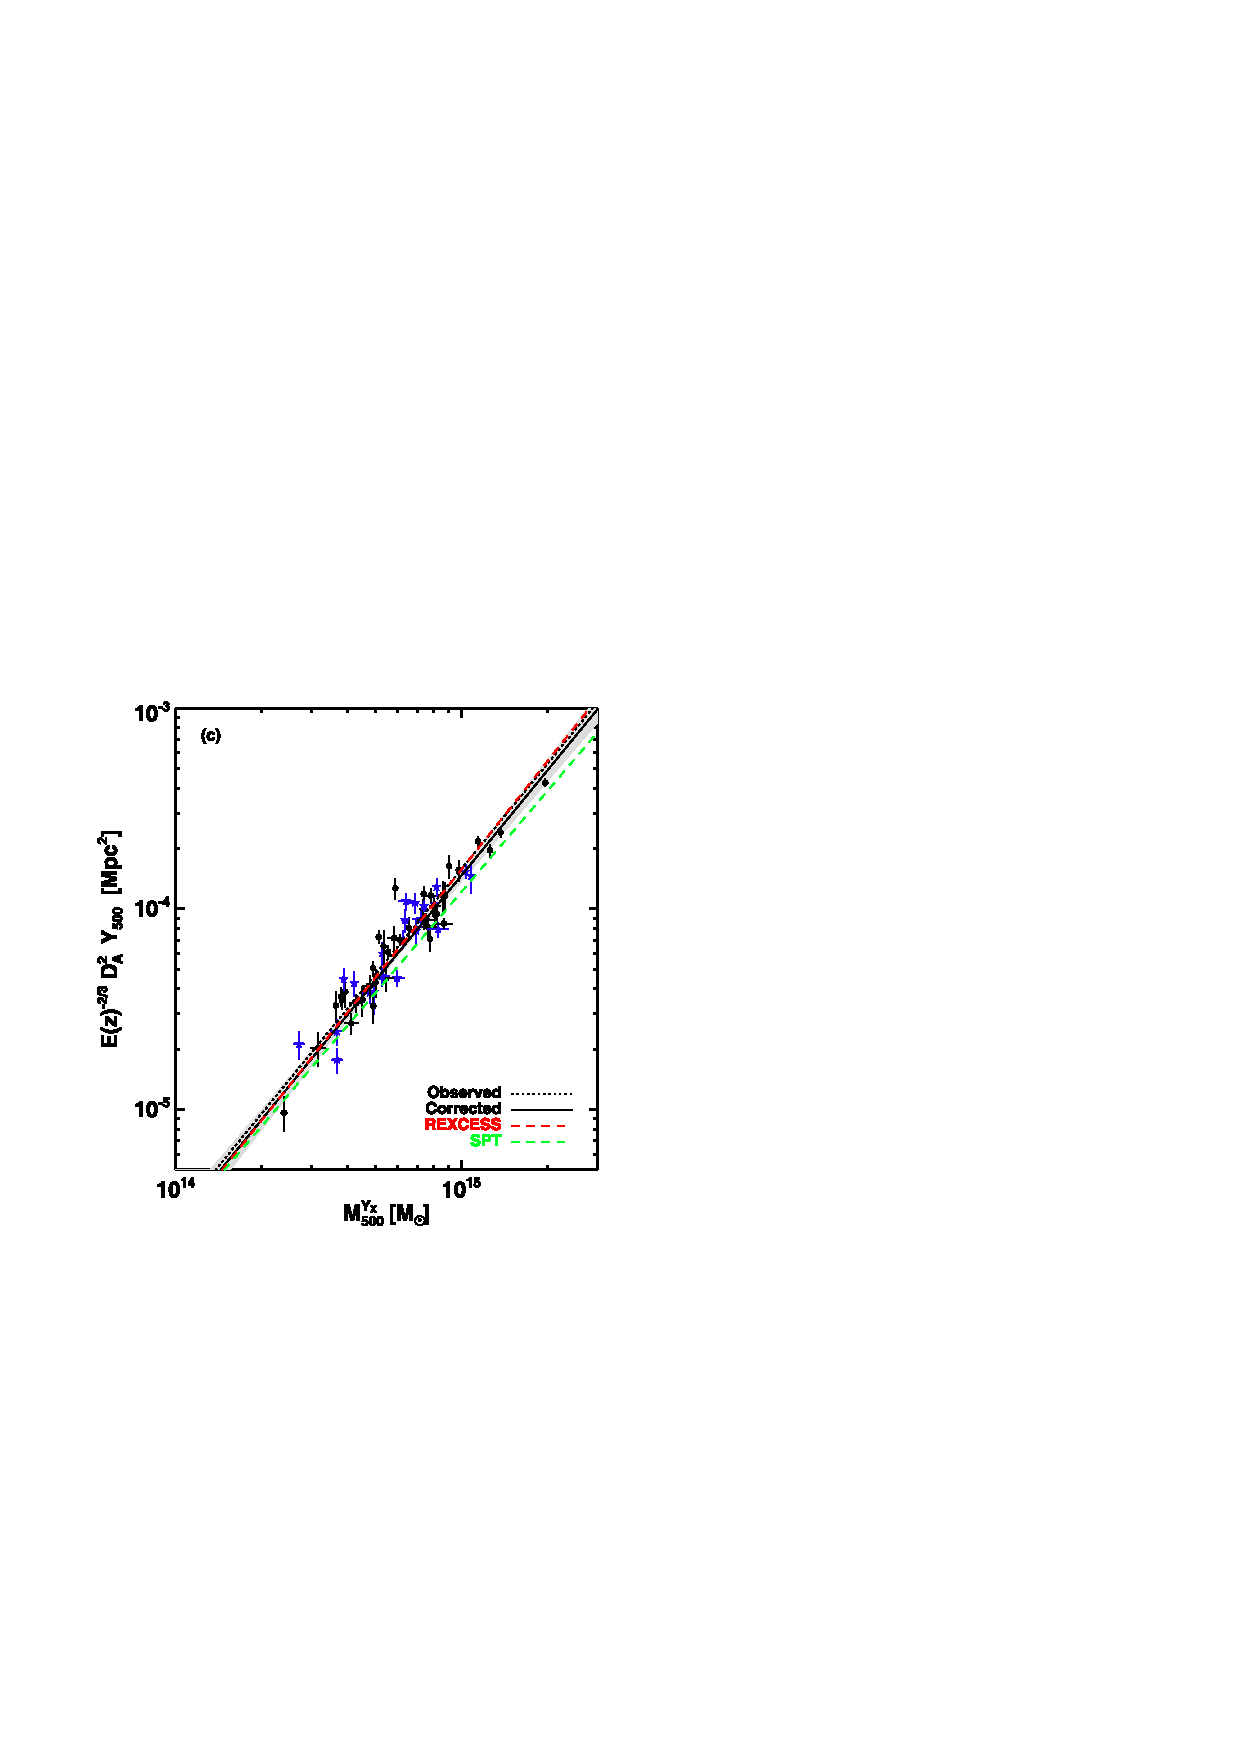
\includegraphics[width=.5\linewidth]{Figures/Chap_scaling/planck.pdf}
    \caption{
        Mesure de la relation d'échelle $Y_{500}-M_{500}$ par la collaboration \textit{Planck}.
        Chaque point représente un amas de galaxies.
        La relation ajustant le mieux les données est présentée en noir, et comparée aux relations issues des analyses de l'échantillon REXCESS en X (rouge, \cite{arnaud_universal_2010}) et SPT en SZ (vert, \cite{andersson_x-ray_2011}).
        Figure extraite de \cite{planck_collaboration_planck_2011}.
    }
    \label{fig:scaling:planck}
\end{figure*}

Plus récemment, dans le cadre de l'étude CoMaLit, \myciteauthor{sereno_comalit_2015-1} ont utilisé les valeurs de paramètre de Compton intégré issues du catalogue d'amas de la collaboration \textit{Planck} pour mesurer la relation d'échelle en utilisant plusieurs mesures de masses différentes.
Sont notamment comparés les résultats obtenus pour des masses d'amas mesurées en X, mais également par lentillage gravitationnel.
La méthodologie employée pour l'ajustement des relations est basée sur un modèle bayésien hiérarchique, similaire à celui que nous utiliserons au cours de ce chapitre.
Comme nous le verrons en section \ref{sec:scaling:model}, cette approche permet de tenir compte des différents effets systématiques affectant l'ajustement de la relation d'échelle.
Les résultats obtenus par \myciteauthor{sereno_comalit_2015-1} sont similaires à ceux de la collaboration \textit{Planck} lors de l'analyse du même échantillon, mais avec des incertitudes augmentées d'environ un ordre de grandeur, correspondant à une prise en compte plus complète des incertitudes.

À la date de l'écriture de cette thèse, il n'existe pas d'étude ayant mesuré la relation d'échelle $Y_{500}-M_{500}$ en utilisant la combinaison d'observations SZ à haute résolution et X, ni d'étude ayant réalisé cette mesure à des redshifts supérieurs à 0.5.
Le grand programme SZ de NIKA2 représente donc une avancée majeure pour la connaissance du lien entre cette observable SZ et la masse des amas de galaxies.

% ===================================================================================== %
\section{Modélisation probabiliste de la relation d'échelle}
\label{sec:scaling:model}

Cette section détaille la modélisation probabiliste de la relation d'échelle liant $Y_{500}$ et $M_{500}$, et les différentes subtilités devant être prises en compte lors de l'ajustement de ce modèle sur des données.
Elle est inspirée du travail de \myciteauthor{sereno_bayesian_2016}, qui offre un cadre probabiliste à l'étude des relations linéaires dans le contexte de l'astronomie.
L'ajustement d'une telle relation peut être effectué de plusieurs façons; nous nous intéressons ici au cadre général d'un modèle \textit{errors in variable} (\cite{dellaportas_bayesian_1995, dagostini_fits_2005, feigelson_modern_2012}, chapitre 4.3 de \cite{hilbe_bayesian_2017}).
Ce modèle est caractérisé par une approche bayésienne hiérarchique de la régression linéaire, dans laquelle le modèle est découpé en plusieurs sous-modèles, chacun caractérisé comme une distribution de probabilité.
Des approches fréquentistes permettant de répondre aux besoins créés par les caractéristiques des jeux de données d'astronomie existent également, comme l'algorithme BCES (\textit{bivariate correlated errors and scatter}, \cite{akritas_linear_1996}).
De telles approches sont décrites dans la revue d'\myciteauthor{andreon_measurement_2013}.

% ------------------------------------------------------------------------------------- %
\subsection{Relation linéaire masse-observable}

À l'instar de la relation $Y_{500} - M_{500}$, la plupart des relations d'échelle masse-observable utilisées en cosmologie avec des amas de galaxies sont des lois de puissance évoluant avec le redshift.
De telles relations peuvent prendre une forme linéaire en s'intéressant aux logarithmes de la masse et de l'observable; on peut alors écrire
\begin{equation}
    \label{eq:scaling:general}
    Y = \alpha_\yz + \beta_\yz Z + \gamma \, T(z) + \delta \, T(z) \, Z,
\end{equation}
où $T(z) = \log_{10} E(z)$. \\
Dans cette équation, $Y$ est le logarithme de l'observable, et $Z$ celui de la masse\footnotemark.
\footnotetext{Par la suite, nous parlerons d'observable et de masse pour $Y$ et $Z$ par simplicité.}
Dans la littérature statistique traitant des régressions linéaires, $Z$ est nommée variable latente ou indépendante, tandis que $Y$ est nommée variable de réponse.
$\alpha_\yz$ et $\beta_\yz$ sont l'ordonnée à l'origine et la pente de la relation, et $\gamma$ et $\delta$ paramétrisent l'évolution avec le redshift de la normalisation et de la pente de la relation. \\
En procédant par association entre les équations (\ref{eq:sz_scaling}) et (\ref{eq:scaling:general}), on voit qu'elles sont équivalentes pour:
\begin{align}
    \nonumber Y &\equiv \log_{10} \left[\frac{Y_{500}}{10^{-4} \,\unit{Mpc^2}}\right], \\
    \nonumber Z &\equiv \log_{10} \left[\frac{M_{500}}{3 \times 10^{14} \,M_\odot}\right], \\
    \nonumber \gamma &= 2/3, \\
    \delta &= 0.
    \label{eq:scaling:sz}
\end{align}
Ainsi, l'équation (\ref{eq:scaling:general}) est plus générale que (\ref{eq:sz_scaling}), puisque la possibilité de considérer des valeurs de $\gamma \neq 2/3$ et $\delta \neq 0$ permet d'étudier l'écart à l'autosimilarité et l'évolution d'une relation d'échelle avec le redshift.

L'ajustement d'une relation d'échelle est donc celui d'une relation linéaire.
Toutefois, plusieurs caractéristiques des données et du modèle rendent cet ajustement complexe.
Il est notamment important de tenir compte de l'existence d'une dispersion intrinsèque autour de la relation d'échelle, de la différence entre estimateur de masse et masse réelle des amas, ainsi que des incertitudes de mesures sur les deux quantités, qui peuvent être corrélées.
Ces caractéristiques constituent les sous-modèles du modèle bayésien hiérarchique, que nous décrivons ci-après.

\subsubsection{Dispersion intrinsèque} % ---------------------------------------------- %
\label{sec:scaling:int_scat}

En réalité, la relation masse-observable ne suit pas parfaitement une loi de puissance.
Dans le cas de la relation $Y_{500} - M_{500}$, il existe un grand nombre de processus physiques complexes qui peuvent altérer le contenu en énergie thermique d'un amas sans être associés à un changement de masse.
Ainsi, l'équation (\ref{eq:scaling:general}) n'est qu'une tendance, et pas une relation strictement suivie par tous les amas de galaxies.
On parle alors de dispersion intrinsèque autour de la relation.

La dispersion intrinsèque d'une relation d'échelle revêt une importance capitale dans l'exploitation cosmologique d'un échantillon d'amas de galaxies.
En effet, sa valeur peut être interprétée comme une mesure de la qualité d'une observable en tant que \textit{proxy} de masse\footnotemark.
\footnotetext{Le terme de \textit{proxy} de masse fait référence à une observable corrélée à la masse, qui peut être utilisée pour prédire la masse d'un amas à l'aide d'une relation d'échelle.}
Ainsi, une relation masse-observable très dispersée est caractéristique d'une observable peu corrélée à la masse.
L'étalonnage en masse des amas est alors peu précis, et les contraintes sur les paramètres cosmologiques sont moins fortes.
Ainsi, la valeur de la dispersion intrinsèque est un paramètre d'intérêt de l'ajustement d'une relation d'échelle, au même titre que sa pente et son ordonnée à l'origine.

La prise en compte de l'existence d'une dispersion intrinsèque autour de la relation d'échelle n'est pas triviale, et ne peut pas être obtenue simplement en généralisant un estimateur de $\chi^2$.
Prenons l'exemple de l'ajustement d'un groupe de points $\{x_i, y_i\}, i \in [1\dots N]$ par une droite d'équation $f(x) = \alpha + \beta x$.
Les valeurs des paramètres $\alpha$ et $\beta$ décrivant le modèle en meilleur accord avec les données peuvent être trouvées en minimisant:
\begin{equation}
    \label{eq:scaling:chi2}
    \chi^2 = \frac{1}{N} \sum_i \frac{\big(y_i - (\alpha + \beta x_i) \big)^2}{\sigma_{y,i}^2},
\end{equation}
où $\sigma_{y, i}$ représente l'incertitude de mesure sur la valeur $y_i$. \\
Afin de tenir compte d'une dispersion intrinsèque $\sigma_{\rm int.}$ autour de la relation, on peut modifier l'équation (\ref{eq:scaling:chi2}) de sorte à inclure la dispersion intrinsèque au dénominateur, soit $\sigma_{y,i}^2 \rightarrow \sigma_{y,i}^2 + \sigma_{\rm int.}^2$.
Si ce remplacement permet en effet de tenir compte de l'existence d'une dispersion intrinsèque, il ne permet pas de mesurer la valeur de ce paramètre: la valeur de $\sigma_{\rm int.}$ minimisant l'équation (\ref{eq:scaling:chi2}) est $\sigma_{\rm int.} \rightarrow \infty$.

Il est possible de tenir compte du caractère non-déterministe de la relation masse-observable en la modélisant non pas comme une relation stricte, mais comme une distribution de probabilité.
On peut notamment considérer une distribution gaussienne:
\begin{equation}
    \label{eq:scaling:general_pdf}
    P(\yzb) = \N \left(\alpha_\yz + \beta_\yz Z + \gamma \, T(z) + \delta \, T(z) \, Z, \sigma_\yz^2 \right),
\end{equation}
où $\N(\mu, \nu)$ est la distribution normale de moyenne $\mu$ et variance $\nu$. \\
On note $\sigma_\yz$ la dispersion intrinsèque de la relation d'échelle, encapsulant la variabilité des valeurs d'observable $Y$ pouvant être associés à une valeur de masse $Z$.
Cette équation constitue l'un des sous-modèles permettant de structurer le modèle hiérarchique de relation d'échelle.

\subsubsection{Estimateurs de masse} % ------------------------------------------------ %
\label{sec:eddington_biases}

Comme nous l'avons discuté au chapitre \ref{chap:amas}, la masse hydrostatique mesurée par combinaison d'observations X et SZ est un estimateur biaisé de la vraie masse d'un amas.
Aucun estimateur de masse n'est parfait.
En effet, la masse hydrostatique est un estimateur certes biaisé, mais peu dispersé; à l'inverse, les estimateurs de masse par lentillage gravitationnel sont moins biaisés, mais plus dispersés (\eg\ \cite{grandis_calibration_2021,sommer_weak_2021}).
Une revue sur les estimateurs de masse d'amas de galaxies, discutant leur justesse et leur précision propre, peut être trouvée en \cite{pratt_galaxy_2019}.

Il est nécessaire de tenir compte des biais et dispersions caractéristiques des estimateurs de masse dans l'étalonnage d'une relation d'échelle.
En effet, l'utilisation d'une relation d'échelle étalonnée à l'aide d'un estimateur de masse biaisé entraînera une estimation biaisée des masses des amas, et donc un biais dans les analyses cosmologiques.
De même, un estimateur de masse dispersé induit un biais sur la pente de la relation d'échelle, un effet connu sous le nom de biais d'Eddington (\cite{eddington_formula_1913, eddington_correction_1940}).
Afin de tenir compte des imperfections caractéristiques de l'estimateur de masse utilisé, on peut définir l'estimateur de masse $X$, relié à la masse réelle de l'amas $Z$ au travers d'une distribution de probabilité:
\begin{equation}
    \label{eq:scaling:mass_estim}
    P(X\,|\,Z) = \N \left(\alpha_{X|Z} + \beta_{X|Z} Z, \sigma_{X|Z}^2\right),
\end{equation}
où $\alpha_{X|Z}$ est le biais de l'estimateur de masse, $\beta_{X|Z}$ quantifie l'évolution de ce biais avec la masse de l'amas, et $\sigma_{X|Z}$ est la dispersion de l'estimateur. \\
Dans le cas de la masse hydrostatique, $\alpha_{X|Z}$ est le biais hydrostatique $b$ discuté en section \mypageref{sec:hse_bias}.
L'équation (\ref{eq:scaling:mass_estim}) constitue un autre des sous-modèles de l'approche hiérarchique.

\subsubsection{Incertitudes de mesure} % ---------------------------------------------- %

La propagation des incertitudes de mesure dans l'ajustement d'une relation d'échelle est également d'une importance capitale (voir \cite{andreon_measurement_2013} pour une revue).
Dans le cadre de l'étude de relations d'échelle masse-observable, la nature des données crée une complication supplémentaire dans l'ajustement.
En effet, les valeurs d'observable et de masse mesurées comportent toutes deux des incertitudes.
Or, il est difficile de réaliser un ajustement comportant des incertitudes à la fois en abscisse et en ordonnée.
Il est toutefois possible d'inclure ces incertitudes dans un estimateur de $\chi^2$.
De la même façon que pour la dispersion intrinsèque, l'équation (\ref{eq:scaling:chi2}) peut être généralisée en remplaçant son dénominateur comme $\sigma_{y,i}^2 \rightarrow \sigma_{y,i}^2 + \beta \sigma_{x, i}^2$.
Tout comme pour l'inclusion d'une dispersion intrinsèque, cette approche conduit à des valeurs de paramètres biaisées, puisque la valeur de $\chi^2$ peut être diminuée avec une augmentation de $\beta$, ce qui crée un biais vers les grandes valeurs de pente.

Le modèle \textit{errors in variable} permet de tenir compte des incertitudes de mesures sur les deux axes de la relation d'échelle et de leur éventuelle corrélation en modélisant chaque point de données (les valeurs de masse et d'observable de chaque amas considéré dans l'ajustement) comme une distribution de probabilités multivariée.
Pour un amas de galaxies $i$, on peut alors écrire:
\begin{equation}
    \label{eq:scaling:pdf_data}
    P(x_i, y_i \,|\, X_i, Y_i) = \N_{\rm 2D}\big(\{X_i, Y_i\}, V_i\big),
\end{equation}
où $x_i$ et $y_i$ sont les valeurs mesurées de l'estimateur de masse et de l'observable, $X_i$ et $Y_i$ sont les vraies valeurs de ces deux grandeurs, et $V_i$ est la matrice de covariance des incertitudes sur $x_i$ et $y_i$. \\
Ainsi, dans cette modélisation de la relation d'échelle, les valeurs réelles des estimateurs de masse et d'observable sont des paramètres de nuisance du modèle.
L'équation (\ref{eq:scaling:pdf_data}) comporte une distribution de probabilité pour chaque point de données $i$, et constitue autant de sous-modèles pour le modèle hiérarchique.

Nous avons vu en section \ref{sec:panco:demo} que \texttt{PANCO2} permettait de mesurer, pour un amas, la distribution de probabilité dans le plan $M_{500}-Y_{500}$ (voir figure \ref{fig:panco2:actlike_integ}).
Ainsi, l'analyse avec \texttt{PANCO2} de tous les amas de galaxies du grand programme SZ de NIKA2 permettra de mesurer pour chaque amas les grandeurs $x_i$, $y_i$, et $V_i$, qui seront les données d'entrée de l'ajustement de la relation d'échelle au travers de l'équation (\ref{eq:scaling:pdf_data}).

% ------------------------------------------------------------------------------------- %
\subsection{Effets de sélection et représentativité}

Nous avons vu dans le chapitre \ref{chap:amas} que la fonction de sélection d'un relevé d'amas devait être prise en compte dans l'exploitation cosmologique de ce dernier, afin de calculer le nombre d'amas observables en fonction des paramètres cosmologiques.
De la même façon, un échantillon d'amas utilisé pour ajuster une relation d'échelle a subi une sélection.
Cette sélection peut avoir un effet important sur l'ajustement de la relation d'échelle, et doit donc être prise en compte.

\subsubsection{Biais de Malmquist} % -------------------------------------------------- %
\label{sec:scaling:malmquist}

L'un des effets de sélection les plus fréquemment rencontrés en astronomie est le biais de Malmquist \cite{malmquist_relations_1922}.
Celui-ci intervient lorsque l'échantillon considéré pour la régression est tronqué à une valeur d'observable minimale.
Il est donc omniprésent en astronomie, puisque les relevés du ciel sont souvent limités en flux du fait de leur sensibilité.
Dans le cadre d'une relation d'échelle masse-observable, il est présent lorsque l'échantillon considéré pour l'ajustement est composé uniquement d'amas dont l'observable est supérieure à un seuil donné.
Ainsi, la significativité de détection, souvent utilisée comme observable corrélée à la masse en optique et SZ (voir section \ref{sec:scaling}, page \pageref{sec:scaling}), est intrinsèquement affectée par le biais de Malmquist, puisque les catalogues construits à partir de cette grandeur sont souvent limités à une valeur seuil.

Le biais de Malmquist se manifeste comme un biais sur les valeurs des paramètres mesurés lors de l'ajustement de relations d'échelle.
Il est lié à une surreprésentation des amas au dessus de la valeur seuil d'observable.
Afin d'illustrer cet effet, un exemple est présenté en figure \ref{fig:malmquist}.
Un ensemble de 100 valeurs de $x$ sont générées aléatoirement à partir d'une distribution log-normale.
Les valeurs de $y$ correspondantes sont générées en considérant une relation linéaire comportant une dispersion intrinsèque, avec les paramètres suivants:
\begin{equation}
    \alpha = 0; \quad \beta = 1; \quad \sigma = 0.25.
\end{equation}
La relation d'échelle correspondante est représentée par une ligne noire pointillée sur le panneau gauche de la figure \ref{fig:malmquist}, et la valeur des paramètres dans le plan $(\alpha, \beta)$  de la même façon dans le panneau droit.
L'ajustement\footnotemark\ des 100 points de cet échantillon permet d'obtenir une relation proche de celle utilisée pour générer les points, représentée par la ligne noire pleine.
Les intervalles de confiance sur les paramètres $\alpha$ et $\beta$ sont représentés en noir sur le panneau gauche de la figure \ref{fig:malmquist}, et sont compatibles avec la vérité.
\footnotetext{La méthode d'ajustement par MCMC sera détaillée en \ref{sec:scaling:mcmc}.}

On considère ensuite seulement les $60$ points correspondant aux valeurs de $y$ les plus élevés, soit, dans cet exemple, les points satisfaisant $y > 0.88$.
Les $40$ points non considérés sont donc les points de valeur de $y$ plus faible que ce seuil, correspondant à la région grisée.
En répétant le même ajustement que celui réalisé précédemment -- qui avait donné la droite noire -- sur les points au-dessus de ce seuil, on obtient une relation d'échelle biaisée, représentée en rouge.
Le biais sur les paramètres $\alpha$ et $\beta$ est clairement visible sur le panneau droit (en rouge également).
La raison de ce biais est la surreprésentation des points au dessus du seuil en $y$.
En effet, du fait de l'existence d'une dispersion intrinsèque, des points de faible valeur de $x$, dont l'observable $y$ aurait été inférieure au seuil en l'absence de dispersion intrinsèque, se retrouvent au dessus du seuil par une fluctuation statistique positive.
À l'inverse, des points de plus grande valeur de $x$ se retrouvent sous le seuil, et donc non-détectés, du fait d'une fluctuation négative.
Par conséquent, l'échantillon détecté comporte une surpopulation de points au dessus de la relation d'échelle réelle, introduisant un biais.
Ce biais peut être compris visuellement grâce à la partie inférieure du panneau gauche de la figure \ref{fig:malmquist}.
Celui-ci représente la différence entre les points de données et relation d'échelles du panneau supérieur et la relation réelle.
On voit clairement la surreprésentation des points au dessus de la relation d'échelle dans la région du seuil en $y$.

\begin{figure*}[t]
    \centering
    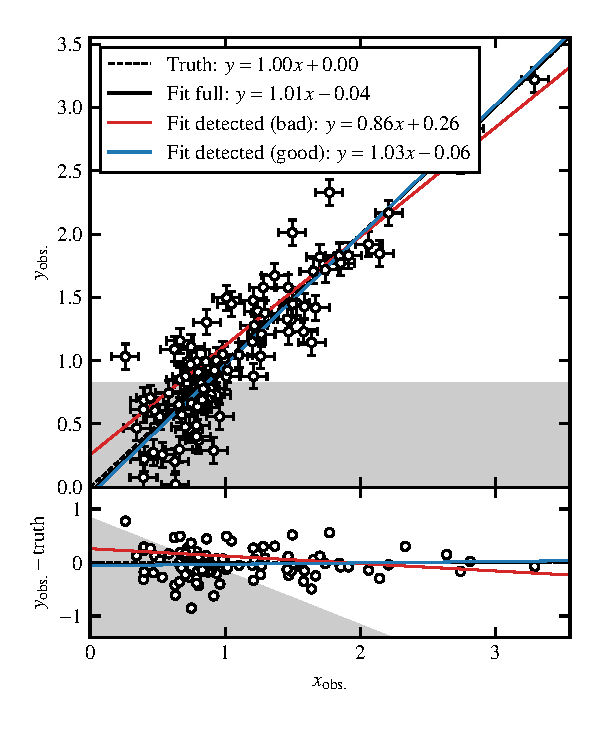
\includegraphics[width=.49\linewidth]{Figures/Chap_scaling/malmquist_effect.pdf}
    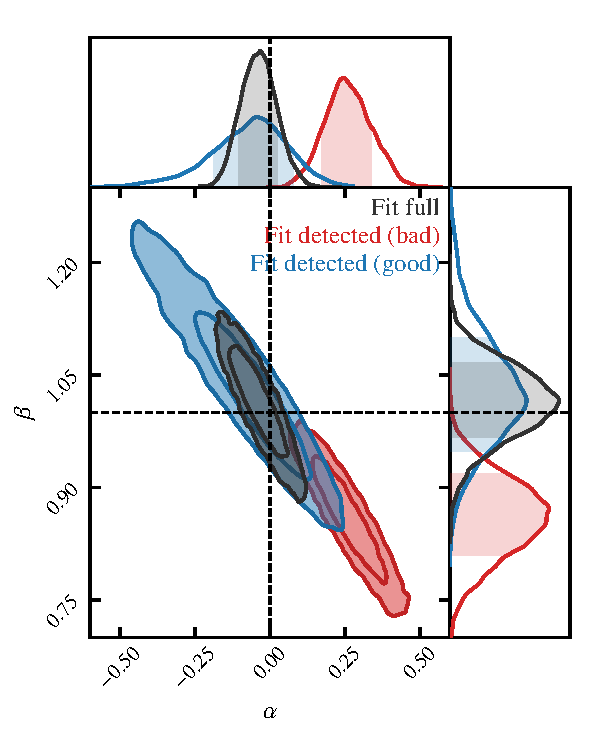
\includegraphics[width=.49\linewidth]{Figures/Chap_scaling/malmquist_effect_2.pdf}
    \caption{
        Illustration du biais de Malmquist dans l'ajustement d'une relation d'échelle.
        \textbf{Gauche:} représentation des données et des relations d'échelles ajustées dans le plan $(x, y)$ (\textit{haut}) et résidus autour de la relation d'échelle réelle (\textit{bas}).
        \textbf{Droite:} intervalles de confiance à $1\sigma$ et $2\sigma$ dans le plan $(\alpha, \beta)$ obtenus par régression.
        Voir texte pour le détail des différentes régressions.
    }
    \label{fig:malmquist}
\end{figure*}

Afin de réaliser un ajustement non-affecté par le biais de Malmquist, il est donc nécessaire de tenir compte de la présence d'une sélection en $y$.
Dans le cadre de la modélisation \textit{errors in variable}, cette prise en compte peut être réalisée en tronquant la distribution de probabilité associée à chaque point de données.
Pour une coupure à une valeur de seuil $y_{\rm th.}$, l'équation (\ref{eq:scaling:pdf_data}) peut être réécrite comme:
\begin{equation}
    \label{eq:scaling:pdf_data_trunc}
    P(x_i, y_i \,|\, X_i, Y_i) \propto \N_{\rm 2D}\big(\{X_i, Y_i\}, V_i\big) \times H(y_i - y_{\rm th.}),
\end{equation}
où $H(x)$ est la fonction de Heaviside, définie comme
\begin{equation}
    H(x) =
        \begin{cases}
            \; 1 \;\text{si}\; x \geqslant 0, \\
            \; 0 \;\text{sinon.}
        \end{cases}
\end{equation}
Cette troncature permet de supprimer toute l'information apportée par les données en dessous du seuil de détection, et donc la surreprésentation des points au dessus de la relation d'échelle réelle.
Les résultats de l'ajustement des points détectés en tenant compte de la troncature (équation \ref{eq:scaling:pdf_data_trunc}) sont représentés en bleu sur la figure \ref{fig:malmquist}.
La droite obtenue est très proche de la relation d'échelle réelle utilisée pour générer les données.
Cette similarité montre que la troncature permet de corriger le biais de Malmquist.

\subsubsection{Distribution de masse} % ----------------------------------------------- %

Parmi les effets de sélection pouvant causer des biais dans l'ajustement d'une relation linéaire, on compte également la modélisation de la distribution de la variable latente $Z$.
Les échantillons de données utilisés pour l'ajustement de relations d'échelle\footnote{Et en général en astronomie.} ne sont en général pas représentatifs de la distribution d'objets dans l'Univers.
Dans le cas des amas de galaxies, les échantillons considérés représentent souvent les amas les plus massifs de l'Univers (puisque ces derniers sont en général plus lumineux), et peuvent surreprésenter les amas possédant certaines propriétés physiques (par exemple les amas à cœur froid en X; voir section \ref{sec:lpsz_sci}, page \pageref{sec:lpsz_sci}).
La méconnaissance de la distribution intrinsèque de la variable latente peut induire des biais sur les paramètres de la relation d'échelle, du fait de la non-représentativité de l'échantillon \cite{kelly_aspects_2007}.
Ces effets sont intimement liés aux biais induits par l'utilisation d'estimateurs dispersés de la variable latente (la masse des amas dans ce contexte), et font donc partie des biais dits d'Eddington discutés en \mypageref{sec:eddington_biases} \cite{eddington_formula_1913,eddington_correction_1940}.

Afin de tenir compte de la différence entre les distributions en masse de l'échantillon et de la population parente (c'est-à-dire tous les amas de l'Univers), il est possible d'inclure la distribution de $Z$ dans la modélisation statistique.
Cette approche a été introduite par \myciteauthor{kelly_aspects_2007} et reprise pour de nombreuses analyses de relations d'échelles masse-observable \cite{sereno_comparing_2015, sereno_bayesian_2016, mantz_gibbs_2016}.
Dans cette approche, la distribution de la variable latente est modélisée comme une somme de $n_{\rm mix}$ gaussiennes pondérées:
\begin{equation}
    \label{eq:scaling:gauss_mix}
    P(Z) = \frac{1}{n_{\rm mix}}\sum_{k=1}^{n_{\rm mix}} \pi_k \, \N(\mu_k, \sigma_k^2),
\end{equation}
où $\mu_k$ et $\sigma_k^2$ représentent les moyennes et variances de la gaussienne $k$, et $\pi_k$ son poids\footnotemark.
\footnotetext{Notons que les paramètres $\pi_k$, $\mu_k$ et $\sigma_k$ pourraient évoluer avec le redshift, mais que nous ne considèrerons pas de telles évolutions.}
Ce dernier peut être interprété comme la probabilité qu'un amas considéré dans un échantillon soit issu de la gaussienne $k$, de sorte à ce que $\sum_k \pi_k = 1$. \\
Les paramètres des gaussiennes $\pi_k$, $\mu_k$ et $\sigma_k$ sont traités comme des paramètres de nuisance du modèle probabiliste de relation d'échelle; les résultats finaux sont marginalisés sur ces paramètres.
L'équation (\ref{eq:scaling:gauss_mix}) représente le dernier sous-modèle du modèle bayésien hiérarchique de la relation d'échelle.

% ===================================================================================== %
\section{Ajustement de la relation d'échelle par MCMC} \label{sec:scaling:mcmc}

La section précédente a permis de détailler la modélisation probabiliste de la relation d'échelle adoptée pour les études menées au cours de cette thèse.
L'objectif de l'ajustement de cette relation est l'obtention de la distribution de probabilité des paramètres d'intérêt de la relation d'échelle conditionnée par les données, $P(\vartheta | D)$.
De même que pour l'ajustement des profils de pression avec \texttt{PANCO2} (voir chapitre \ref{chap:panco}), cette distribution peut être obtenue à partir du théorème de Bayes:
\begin{equation}
    \label{eq:bayes_scaling}
    P(\vartheta \,|\, D) = \frac{P(D \,|\, \vartheta) \; P(\vartheta)}{P(D)},
\end{equation}
où $\vartheta$ est un vecteur représentant les paramètres de l'analyse, $D$ représente les données, c'est-à-dire les valeurs de $(x_i, y_i)$ et leurs covariances $V_i$.
$P(D|\vartheta)$ représente la fonction de vraisemblance comparant le modèle aux données, obtenu par combinaison des équations  (\ref{eq:scaling:pdf_data}), (\ref{eq:scaling:general_pdf}), (\ref{eq:scaling:mass_estim}) et (\ref{eq:scaling:gauss_mix}).
$P(\vartheta)$ représente la distribution \prior\ des paramètres, et $P(D)$ est une constante de normalisation.

Comme nous l'avons vu, le modèle statistique de relation d'échelle est complexe; nous verrons de plus que son ajustement sur des données l'est également.
Par conséquent, les études réalisées au cours de cette thèse se basent sur une librairie existante nommée \texttt{LIRA} (\textit{LInear Regression in Astronomy}, \cite{sereno_bayesian_2016}).
Ce logiciel est disponible publiquement sous forme d'une librairie dans le langage R, dédié aux études statistiques et d'analyse de données.
\texttt{LIRA} permet d'ajuster le modèle probabiliste détaillé dans la section précédente en utilisant un échantillonnage par Monte Carlo à Chaînes de Markov (MCMC).
Cette section détaille la construction de la distribution \prior\ $P(\vartheta)$, et l'échantillonnage de la distribution postérieure $P(\vartheta | D)$ par MCMC.

% ------------------------------------------------------------------------------------- %
\subsection{Distribution de probabilité \prior\ des paramètres}

L'approche bayésienne employée dans l'étude de la relation d'échelle nécessite la construction d'une distribution de probabilité \prior\ pour l'ensemble des paramètres de l'analyse.
Les paramètres sont considérés comme indépendants, de sorte à ce que la distribution \prior\ puisse être écrite comme le produit des distributions \prior\ sur chaque paramètre individuel.

La table \ref{tab:scaling:params} présente un résumé des paramètres du modèle et de leur distribution \prior.
Les distributions choisies sont volontairement peu informatives, de sorte à ce que les résultats de l'ajustement ne soient pas entachés d'erreurs dues à l'inclusion d'une connaissance \prior\ des paramètres erronée.
Pour cela, la distribution uniforme $\mathcal{U}$ est utilisée; elle est définie comme:
\begin{equation}
    \mathcal{U}(x_1, x_2) =
        \begin{cases}
            \; 1/|x_1 - x_2| \;\text{entre}\; x_1 \;\text{et}\; x_2, \\
            \; 0 \;\text{ailleurs.}
        \end{cases}
\end{equation}
Les bornes de cette distribution doivent être finies, sans quoi la distribution \prior\ des paramètres ne peut plus être intégrable à 1, et ne représente donc plus une distribution de probabilité.
Le choix des intervalles $[-10^4, 10^4]$ (ou $[0, 10^4]$ dans le cas des valeurs strictement positives) est arbitraire.
Puisque les grandeurs en jeu dans l'ajustement sont mises à l'échelle (équation \ref{eq:scaling:sz}), ces intervalles sont suffisamment larges pour ne pas exclure de région de l'espace des paramètres pouvant fournir une bonne description des données.

Certains paramètres ne se voient pas attribuer une distribution \prior\ uniforme.
Pour le paramètre de pente $\beta_\yz$, la distribution de Student à un degré de liberté est utilisée:
\begin{equation}
    t_1(x) = \frac{1}{\pi} \big(1 + x^2\big)^{-1}.
\end{equation}
Une distribution $t_1(\beta)$ sur la pente d'une relation linéaire correspond à une distribution uniforme sur l'angle entre cette droite et l'axe des abscisses, $\theta = \arctan(\beta)$.
L'utilisation de la distribution de Student revient donc à l'utilisation d'une distribution \prior\ non-informative en coordonnées polaires.
Ce choix peut donner lieu à des valeurs de pentes moins biaisées vers les grandes valeurs de pente qu'un \prior\ uniforme sur $\beta$ \cite{andreon_measurement_2013,sereno_bayesian_2016}. \\
Un autre groupe de paramètres pour lesquels la distribution \prior\ n'est pas uniforme est l'ensemble des poids des gaussiennes considérées pour la modélisation de la distribution intrinsèque de la variable latente, $\pi_k,\; k \in [0\dots n_{\rm mix}]$.
La distribution adoptée est la distribution de Dirichlet, qui permet à la somme des poids d'être égale à 1. \\
Enfin, les paramètres quantifiant l'évolution de la relation d'échelle avec le redshift sont par défaut fixés à leur valeur autosimilaire, $\gamma=2/3$ et $\delta=0$ (équation \ref{eq:scaling:sz}).

Notons que la distribution \prior\ décrite dans cette section est la distribution par défaut pour un ajustement de relation d'échelle.
Il est possible de spécifier une autre distribution pour chaque paramètre, selon les objectifs de l'analyse.
Lors de la présentation de résultats dans les sections \ref{sec:scaling:valid} et \ref{sec:scaling:lpsz}, les distributions choisies pour chaque paramètre seront spécifiées lorsqu'elles seront différentes des options par défaut.

\begin{table}[t]
    \setlength{\tabcolsep}{15pt}
    \small
    \centering
    \begin{tabular}{c l l}
        \toprule
        Paramètre & Description & Distribution \prior \\
        \midrule
        % -------------------------------------------------------------------------- %
        \midrule
        \multicolumn{3}{c}{\itshape Paramètres d'intérêt: relation $Y=f(Z)$} \\
        \midrule
        $\alpha_\yz$ & Ordonnée à l'origine   & $\mathcal{U}(-10^4, 10^4)$ \\
        $\beta_\yz$  & Pente                  & Student $t_1$ \\
        $\sigma_\yz$ & Dispersion intrinsèque & $\mathcal{U}(0, 10^4)$ \\
        $\gamma$ & Évolution avec le redshift de la normalisation & $\delta(2/3)$ \\
        $\delta$ & Évolution avec le redshift de la pente & $\delta(0)$ \\
        % -------------------------------------------------------------------------- %
        \midrule
        \multicolumn{3}{c}{\itshape Paramètres de nuisance: relation $X=f(Z)$} \\
        \midrule
        $\alpha_{X|Z}$ & Ordonnée à l'origine   & $\delta(0)$ \\
        $\beta_{X|Z}$  & Pente                  & $\delta(1)$ \\
        $\sigma_{X|Z}$ & Dispersion intrinsèque & $\delta(0)$ \\
        % -------------------------------------------------------------------------- %
        \midrule
        \multicolumn{3}{c}{\itshape Paramètres de nuisance: distribution de la variable latente} \\
        \midrule
        $\mu_k$    & Moyennes des gaussiennes    & $\mathcal{U}(-10^4, 10^4)$ \\
        $\sigma_k$ & Dispersions des gaussiennes & $\mathcal{U}(0, 10^4)$ \\
        $\pi_k$    & Poids des gaussiennes       & Dirichlet($n_{\rm mix}$) \\
        \bottomrule
    \end{tabular}
    \caption{%
        Liste des paramètres du modèle statistique de relation d'échelle masse-observable.
        La dernière colonne indique les distributions \prior\ par défaut pour chaque paramètre.
    }
    \label{tab:scaling:params}
\end{table}


% ------------------------------------------------------------------------------------- %
\subsection{Analyse MCMC par échantillonnage de Gibbs}

Nous avons vu dans le chapitre \ref{chap:panco} qu'une analyse par Monte Carlo à Chaînes de Markov (MCMC) permettait d'obtenir un échantillon de la distribution postérieure de probabilité $P(\vartheta | D)$ dans l'espace des paramètres.
Cette approche y est illustrée au travers de l'algorithme de Metropolis-Hastings, représentant l'algorithme de MCMC le plus simple à définir.
Nous avons vu cependant que d'autres algorithmes existaient et fournissaient de meilleures performances pour l'échantillonnage de distributions de probabilités dans un grand nombre de dimensions.
Par exemple, dans \texttt{PANCO2}, l'échantillonneur choisi utilise une variation de l'algorithme de Metropolis-Hastings dont la fonction de proposition évolue avec les itérations.

Pour l'ajustement d'une relation d'échelle, il est utile de faire appel à un autre type d'échantillonnage, plus performant pour un très grand nombre de dimensions.
En effet, l'utilisation de la modélisation \textit{errors in variable} implique le traitement de chacune des grandeurs $X_i$ et $Y_i$ comme des paramètres de nuisance.
Ainsi, pour un échantillon de $N$ amas, l'analyse comporte $2N$ paramètres de nuisance, en plus de ceux du modèle résumés dans la table \ref{tab:scaling:params}.
Pour le grand programme SZ de NIKA2, cela représente un nombre de paramètres de l'analyse de l'ordre de la centaine, alors que l'ajustement des propriétés thermodynamiques d'un amas avec \texttt{PANCO2} n'utilise qu'une dizaine de paramètres.

Afin de répondre à ce besoin, un grand nombre de logiciels dédiés à l'ajustement de relations d'échelle (\eg\ \cite{sereno_bayesian_2016, mantz_gibbs_2016}) font appel à l'échantillonnage de Gibbs (\textit{Gibbs sampling}, voir par exemple le chapitre 11.3 de \cite{gelman_bayesian_2013}).
La principale différence entre cette technique et l'algorithme de Metropolis-Hastings est le fait que le mouvement dans l'espace des paramètres n'est pas fait pour tous les paramètres simultanément, mais par groupe de paramètres.
Un vecteur de paramètres $\vartheta$ à $N$ dimensions peut être divisé en $d$ groupes:
\begin{equation}
    \vartheta = (\vartheta_1, \dots \vartheta_N)
    \rightarrow \theta = (\theta_1, \dots \theta_d)
    = (\{\vartheta_1, \dots \vartheta_{n_1}\}, \{\vartheta_{n_1 + 1} \dots \vartheta_{n_1 + n_2}\}, \dots \{\vartheta_{N - n_d}, \dots \vartheta_N\}),
\end{equation}
où $n_i$ est la dimension du groupe $i$. \\
La procédure itérative générant une chaîne de Markov, détaillée en section \mypageref{sec:mcmc_sampling}, est alors appliquée.
La particularité de l'échantillonnage de Gibbs réside dans le fait qu'à chaque itération, l'échantillonneur boucle sur les $d$ groupes pour proposer un mouvement dans l'espace des paramètres groupe par groupe, plutôt que pour tous les paramètres simultanément.
De plus, le mouvement d'un groupe de paramètres est conditionné par celui des autres paramètres, afin de tenir compte des corrélations entre les paramètres de groupes différents.
Dans le cas du modèle bayésien hiérarchique utilisé ici, les groupes de paramètres sont définis en fonction du sous-modèle auquel ils appartiennent.
Par exemple, un groupe est constitué par les paramètres d'intérêt de la relation d'échelle (équation \ref{eq:scaling:general_pdf}); un autre est consacré aux caractéristiques de l'estimateur de masse (équation \ref{eq:scaling:mass_estim}), etc.
La procédure employée pour générer un pas du MCMC dans le cas d'une régression linéaire utilisant la modélisation \textit{errors in variable} est décrite dans la section 6.2.1 de \cite{kelly_aspects_2007}, et comporte 18 étapes qui ne seront pas détaillées ici.

L'échantillonnage de Gibbs est un algorithme MCMC qui produit des chaînes de Markov, c'est-à-dire un échantillonnage de la distribution postérieure de probabilités dans l'espace des paramètres.
Il offre une grande performance au vu du nombre important de paramètres dans l'analyse.
L'échantillonnage réalisé dans \texttt{LIRA} utilise le logiciel JAGS\footnote{\textit{Just Another Gibbs Sampler}, \url{https://mcmc-jags.sourceforge.io/}}, dédié à l'échantillonnage de Gibbs pour des modèles bayésiens structurels.
La marginalisation sur les paramètres de nuisance permet d'obtenir la distribution de probabilité des paramètres d'intérêt au vu des données.
Cette distribution permet alors de calculer la probabilité $P(\yzb)$ qu'un amas de masse $Z$ soit détectable avec une valeur d'observable $Y$.
Comme nous l'avons vu en section \mypageref{sec:cluster_nbcount}, cette probabilité peut être utilisée pour l'étalonnage en masse d'un échantillon d'amas de galaxies en vue de son exploitation cosmologique (équations \ref{eq:nbcount_obs}, \ref{eq:nbcount_sel}).

% ===================================================================================== %
\section{Validation sur données simulées}
\label{sec:scaling:valid}

Nous avons vu dans les sections précédentes que le modèle bayésien hiérarchique utilisé dans cette étude pouvait tenir compte de plusieurs spécificités des jeux de données d'astronomie, et que l'ajustement pouvait être fait à l'aide de la librairie \texttt{LIRA}.
Afin de tester la capacité de \texttt{LIRA} à livrer des mesures justes des paramètres d'une relation linéaire, nous commençons par générer des jeux de données simples, comportant les différentes caractéristiques développées en section \mypageref{sec:scaling:model}.
Ces jeux de données n'ont pas vocation à être des réalisations réalistes pour des relations d'échelle masse-observable; de telles analyses seront présentées par la suite.

% ------------------------------------------------------------------------------------- %
\subsection{Incertitudes de mesure et dispersion intrinsèque}
\label{sec:scaling:valid1}

Nous commençons par générer des données simples, en considérant la présence d'incertitudes de mesures décorrelées sur les deux axes, et l'existence d'une dispersion intrinsèque.
Un total de cent points $i$ sont générés de la façon suivante:
\begin{align}
    \nonumber Z_i &\sim \N\ (0, 1); \\
    \nonumber X_i &\sim \N\ (\alpha_{X|Z} + Z_i, \sigma_{X|Z}^2) \quad \text{(soit $\beta_{X|Z} = 1$)}; \\
    \nonumber Y_i &\sim \N\ (\alpha_\yz + \beta_\yz Z_i, \sigma_\yz^2); \\
    \nonumber x_i &\sim \N\ (X_i, 0.01); \\
              y_i &\sim \N\ (Y_i, 0.01),
              \label{eq:scaling:sim_sample_valid}
\end{align}
où $A \sim B$ signifie \guillemotleft $A$ est distribué suivant $B$ \guillemotright, et les valeurs utilisées pour les paramètres sont consignées en table \ref{tab:scaling:valid}. \\
L'échantillon des $(x_i, y_i)$ est ensuite ajusté avec \texttt{LIRA}, en considérant les distributions \prior\ par défaut (voir table \ref{tab:scaling:params}), sauf pour les paramètres de la relation $X = f(Z)$ qui sont fixés.
La liste des valeurs réelles des paramètres et de leurs distributions \prior\ pour cette analyse est donnée en table \ref{tab:scaling:valid}.

L'objectif de cette analyse est de pouvoir estimer si les paramètres d'intérêt de la relation d'échelle sont correctement reconstruits par \texttt{LIRA}.
Pour cela, nous définissons deux grandeurs permettant de quantifier le biais des estimateurs de paramètres donnés par \texttt{LIRA}: pour un paramètre $\vartheta$,
\begin{align}
    \nonumber \xi_\vartheta &\equiv \frac{{\rm Med} \big[\vartheta_i\big]_i - \hat{\vartheta}}{|\hat{\vartheta}|}, \\
    \zeta_\vartheta &\equiv \frac{{\rm Med} \big[\vartheta_i\big]_i - \hat{\vartheta}}{\sqrt{{\rm Var}\big[\vartheta_i\big]_i}},
    \label{eq:scaling:xi_zeta}
\end{align}
où $\vartheta_i$ représente l'échantillon $i$ de la chaîne de Markov sur le paramètre $\vartheta$, et $\hat{\vartheta}$ est la valeur réelle du paramètre, utilisée pour générer l'analyse.
Les opérations ${\rm Med}[\dots]_i$ et ${\rm Var}[\dots]_i$ représentent la médiane et la variance des échantillons. \\
Ces deux grandeurs permettent de comparer la valeur de la médiane des chaînes, utilisée comme estimateur des paramètres, à la valeur réelle du paramètre.
$\xi$ permet d'exprimer le biais de l'estimateur en fraction de la valeur réelle, tandis que $\zeta$ mesure le biais par rapport à l'écart-type des chaînes, et peut donc être interprété comme la significativité du biais.
Enfin, la variance des chaînes est également importante, puisqu'elle permet de quantifier l'incertitude sur ce paramètre.
On définit alors l'écart-type relatif sur un paramètre comme:
\begin{equation}
    \label{eq:scaling:eta}
    \eta_\vartheta \equiv \frac{\sqrt{{\rm Var}\big[\vartheta_i\big]_i}}{|\hat{\vartheta}|}.
\end{equation}

La procédure de génération d'un échantillon aléatoire et d'ajustement d'une relation linéaire avec \texttt{LIRA} est répété 5000 fois.
L'objectif est la mesure des performances de \texttt{LIRA} à travers l'étude de la distribution des paramètres $\xi_\vartheta$, $\zeta_\vartheta$ et $\eta_\vartheta$ pour chaque paramètre d'intérêt $\vartheta$.
Pour chaque réalisation, ces trois grandeurs sont calculées pour chacun des paramètres d'intérêt $\alpha_\yz$, $\beta_\yz$, et $\sigma_\yz$.
Les valeurs moyennes pour chacun des paramètres d'intérêt de la relation d'échelle sont présentées dans la partie droite de la table \ref{tab:scaling:valid}.
On voit que l'analyse permet d'obtenir des résultats très peu biaisés pour tous les paramètres, soit $\xi \ll 100$\% et $\zeta \ll 1\sigma$ pour tous les paramètres d'intérêt.
La dispersion des estimateurs des paramètres $\eta$ est également calculée.
Les données utilisées pour la validation n'ayant pas pour but d'être réalistes, la valeur de $\eta$ ne présente pas d'intérêt majeur, si ce n'est d'être comparée entre les différentes analyses.
En effet, nous verrons par la suite que l'ajout de paramètres de nuisance dans l'analyse augmente la dispersion des estimateurs des paramètres d'intérêt.

\begin{table}[t]
    \setlength{\tabcolsep}{10pt}
    \small
    \centering
    \begin{tabular}{c c c c c c}
        \toprule
        \multirow{2}{*}{Paramètre $\vartheta$} & \multicolumn{2}{c}{Paramètres de l'analyse} & \multicolumn{3}{c}{Résultats} \\
        \cmidrule(lr){2-3} \cmidrule(lr){4-6}
        & Valeur d'entrée & Distribution \prior
        & $\xi_\vartheta$ [\%] & $\zeta_\vartheta \; [\sigma]$ & $\eta_\vartheta$ [\%] \\
        % ========================================================================== %
        \midrule
        \multicolumn{6}{c}{\textit{Dispersion intrinsèque seulement} (section \ref{sec:scaling:valid1})} \\
        \midrule
        % -------------------------------------------------------------------------- %
        $\alpha_\yz$ & $1   $ & $\mathcal{U}(-10^4, 10^4)$
                       & $-0.03$  & $-0.02$  & $1.74$ \\
        $\beta_\yz$  & $1   $ & Student $t_1$
                       & $0.03$  & $0.01$  & $1.76$ \\
        $\sigma_\yz$ & $0.5 $ & $\mathcal{U}(0, 10^4)$
                       & $-4.88$  & $-0.13$  & $23.87$ \\
        % ========================================================================== %
        \midrule
        \multicolumn{6}{c}{\textit{Estimateur de masse dispersé} (section \ref{sec:scaling:valid2})} \\
        \midrule
        % -------------------------------------------------------------------------- %
        $\alpha_\yz$ & $1   $ & $\mathcal{U}(-10^4, 10^4)$
                       & $0.27$  & $0.00$  & $2.11$ \\
        $\beta_\yz$  & $1   $ & Student $t_1$
                       & $-0.99$  & $-0.01$  & $2.39$ \\
        $\sigma_\yz$ & $0.5 $ & $\mathcal{U}(0, 10^4)$
                       & $-4.94$  & $-0.13$  & $43.70$ \\
        % -------------------------------------------------------------------------- %
        $\sigma_{X|Z}$ & $0.1 $ & $\mathcal{U}(0, 10^4)$ & -- & -- & -- \\
        % ========================================================================== %
        \midrule
        \multicolumn{6}{c}{\textit{Estimateur de masse biaisé} (section \ref{sec:scaling:valid3})} \\
        \midrule
        % -------------------------------------------------------------------------- %
        $\alpha_\yz$ & $1   $ & $\mathcal{U}(-10^4, 10^4)$
                       & $0.02$  & $0.00$  & $5.88$ \\
        $\beta_\yz$  & $1   $ & Student $t_1$
                       & $0.04$  & $0.02$  & $1.76$ \\
        $\sigma_\yz$ & $0.5 $ & $\mathcal{U}(0, 10^4)$
                       & $-4.91$  & $-0.13$  & $23.86$ \\
        % -------------------------------------------------------------------------- %
        $\alpha_{X|Z}$ & $0.8 $ & $\mathcal{U}(0.6, 1)$ & -- & -- & -- \\
        % ========================================================================== %
        \midrule
        \multicolumn{6}{c}{\textit{Données tronquées} (section \ref{sec:scaling:valid4})} \\
        \midrule
        % -------------------------------------------------------------------------- %
        $\alpha_\yz$ & $1   $ & $\mathcal{U}(-10^4, 10^4)$
                       & $-2.08$  & $-0.56$  & $3.47$ \\
        $\beta_\yz$  & $1   $ & Student $t_1$
                       & $1.79$  & $0.53$  & $3.26$ \\
        $\sigma_\yz$ & $0.5 $ & $\mathcal{U}(0, 10^4)$
                       & $-14.15$  & $-0.58$  & $24.84$ \\
        % ========================================================================== %
        \bottomrule
    \end{tabular}
    \caption{%
        Liste des valeurs d'entrée des paramètres, de leurs distributions \prior\ et des résultats pour les analyses de validation présentées en section \ref{sec:scaling:valid}.
        La distribution \prior\ des paramètres non-répertoriés dans cette table est celle par défaut (table \ref{tab:scaling:params}).
        Lorsqu'elles ne sont pas précisées, les valeurs d'entrée des paramètres $\alpha_{X|Z}$ et $\sigma_{X|Z}$ sont nulles.
        Les biais et dispersions des estimateurs des paramètres $\alpha_{X|Z}$ et $\sigma_{X|Z}$ ne sont pas répertoriés car ceux-ci sont des paramètres de nuisance, dont les contraintes ne sont pas l'objectif de l'analyse.
    }
    \label{tab:scaling:valid}
\end{table}

% ------------------------------------------------------------------------------------- %
\subsection{Estimateur de masse dispersé}
\label{sec:scaling:valid2}

La procédure présentée en \ref{sec:scaling:valid1} a permis de confirmer que l'estimation des paramètres d'intérêt de la relation d'échelle n'était pas biaisée dans le cas d'une relation d'échelle comportant des incertitudes sur la variable latente et sur la réponse, et une dispersion intrinsèque non-nulle.
Nous cherchons ensuite à généraliser la validation aux cas de données plus complexes.
Nous commençons par considérer un estimateur de la variable latente dispersé, c'est-à-dire $\sigma_{X|Z} \neq 0$.
Cette dispersion correspond, dans le cas de l'étude d'une relation masse-observable, à l'utilisation d'un estimateur dispersé de la masse d'un amas de galaxies, comme la masse mesurée par lentillage gravitationnel.
Le paramètre $\sigma_{X|Z}$ devient donc un paramètre de nuisance dans l'ajustement, plutôt que d'être fixé comme nul dans la section \ref{sec:scaling:valid1}.
Si cette dispersion n'est pas prise en compte dans l'analyse, elle génère un biais de type Eddington \cite{eddington_formula_1913,eddington_correction_1940}.

Les paramètres de l'analyse, leur distribution \prior\ et les résultats pour les estimateurs de biais $\xi$ et $\zeta$ et de dispersion $\eta$ sont présentées en table \ref{tab:scaling:valid}.
Tout comme dans la section précédente, on voit que les estimateurs pour les paramètres d'intérêt de la relation d'échelle sont très peu biaisés.
En revanche, on voit que la dispersion des paramètres $\eta$ augmente avec l'ajout de $\sigma_{X|Z}$ comme paramètre de nuisance.
Cette augmentation de la dispersion des estimateurs correspond à la propagation de l'incertitude sur le paramètre ajouté.
Elle montre donc l'effet de la prise en compte d'incertitudes systématiques dans l'analyse.
L'ajout de paramètres de nuisance permet donc d'augmenter la justesse des estimateurs -- dans ce cas, en corrigeant le biais d'Eddington -- au détriment de leur précision.
Il est donc important de procéder avec précaution lors de l'ajout de paramètres de nuisances dans l'analyse, au risque d'augmenter artificiellement les incertitudes sur les paramètres d'intérêt.

% ------------------------------------------------------------------------------------- %
\subsection{Estimateur de masse biaisé}
\label{sec:scaling:valid3}

Nous nous intéressons ensuite à l'ajustement d'une relation d'échelle utilisant un estimateur biaisé pour la variable latente.
Ce cas correspond à une valeur non-nulle du paramètre $\alpha_{X|Z}$, qui devient donc un paramètre de l'analyse.
Dans le cas de l'étude d'une relation masse-observable, ce biais correspond à l'utilisation d'un estimateur de masse biaisé, par exemple la masse hydrostatique, dont le biais a été décrit en \mypageref{sec:hse_bias}.

Nous avons choisi d'adopter un \prior\ informatif sur le biais de l'estimateur de variable latente, avec une distribution uniforme étroite centrée sur la valeur réelle du biais utilisé.
En effet, il est possible de mesurer le biais hydrostatique, et les analyses de données et de simulations indiquent que sa valeur est comprise entre $0.6$ et $1$ (voir figure \ref{fig:hse_bias}).
Ainsi, l'utilisation d'un \prior\ informatif est justifiée, et permet de réduire l'espace des paramètres sur la base d'arguments physiques.
Or, comme nous l'avons vu dans la section précédente, l'ajout de paramètres de nuisance diminue la précision des estimateurs de paramètres obtenus par l'ajustement de relations d'échelle.

Les résultats de l'analyse sont consignés dans la troisième partie de la table \ref{tab:scaling:valid}.
Les valeurs moyennes des biais $\xi$ et $\zeta$ nous montrent que les estimateurs des paramètres d'intérêt ne sont pas biaisés.
Les valeurs de dispersions $\eta$ montrent également que les estimateurs sont aussi précis que ceux pour des estimateurs de masse non-biaisés et non-dispersés (section
\ref{sec:scaling:valid1}), sauf pour le paramètre $\alpha_\yz$, dont l'estimateur est trois fois moins précis.
Ainsi, une méconnaissance du biais sur les estimateurs de masse entraîne une imprécision sur la valeur de l'ordonnée à l'origine de la relation masse-observable.

% ------------------------------------------------------------------------------------- %
\subsection{Données tronquées}
\label{sec:scaling:valid4}

La procédure de correction du biais de Malmquist présentée en section \mypageref{sec:scaling:malmquist} est également testée.
Comme l'a montré la figure \ref{fig:malmquist}, l'ajustement d'une relation sur des données tronquées à une valeur d'observable mène à un biais sur les estimateurs des paramètres si cette troncature n'est pas prise en compte.
Afin de s'assurer que les estimateurs des paramètres d'intérêt de la relation d'échelle sont effectivement non-biaisés lorsque la coupure est prise en compte, nous répétons l'analyse réalisée en section \ref{sec:scaling:valid1} avec des échantillons tronqués.
Pour cela, des échantillons de 200 points sont créés en utilisant la procédure décrite dans l'équation (\ref{eq:scaling:sim_sample_valid}), dont seuls sont conservés les points $i$ dont la valeur d'observable mesurée satisfait $y_i > 1$.
Cette coupure permet de créer des échantillons d'environ 100 points, comparables à ceux utilisés dans les tests précédents.
L'ajustement est ensuite réalisé en considérant la coupure au travers de l'équation (\ref{eq:scaling:pdf_data_trunc}).

Les résultats sont consignés dans la table \ref{tab:scaling:valid}.
Les estimateurs des paramètres d'intérêt sont légèrement plus biaisés que lors de l'ajustement d'une relation sur des échantillons non-affectés par une sélection.
Toutefois, ces biais restent faibles et peu significatifs, avec des valeurs de $\zeta$ de l'ordre de $0.5\sigma$.
La dispersion $\eta$ des estimateurs de la pente et de l'ordonnée à l'origine de la relation d'échelle est également augmentée, par un facteur d'environ deux.

% ------------------------------------------------------------------------------------- %
\subsection*{Conclusions}

Les différentes caractéristiques des jeux de données utilisés pour l'ajustement de relations d'échelle masse-observable peuvent être pris en compte par le modèle probabiliste présenté en section \ref{sec:scaling:model}.
L'ajustement de ce modèle avec \texttt{LIRA} permet d'obtenir des estimateurs peu biaisés des paramètres d'intérêt de la relation d'échelle.
La dispersion de ces estimateurs comprend la propagation des effets systématiques, qui sont considérés par l'ajout de paramètres de nuisance dans l'ajustement.
Dans une analyse cosmologique, cette dispersion implique des contraintes moins fortes sur les paramètres cosmologiques.
Il est donc utile de s'interroger en amont sur la pertinence physique des différents paramètres de nuisance utilisés, afin de pouvoir éventuellement diminuer l'espace des paramètres accessible et ainsi augmenter la précision des analyses, sans pour autant compromettre leur justesse.

% ===================================================================================== %
\section{Application au grand programme SZ de NIKA2}
\label{sec:scaling:lpsz}

L'estimation des paramètres de la relation d'échelle liant l'observable SZ $Y_{500}$ et la masse $M_{500}$ est l'un des enjeux majeurs du grand programme SZ de NIKA2.
La procédure d'ajustement développée et testée dans ce chapitre a pour objectif de fournir une estimation juste et précise de ces paramètres à partir des mesures de $Y_{500}$ et $M_{500}$ effectuées à partir des observations NIKA2, et plus particulièrement grâce au logiciel \texttt{PANCO2}, comme décrit en section \mypageref{sec:panco:integrated_qties}.
Dans cette section, nous quantifions le biais et la précision des estimateurs des paramètres de la relation d'échelle au moyen de simulations d'échantillons d'amas réalistes, similaires à celui du grand programme SZ.

% ------------------------------------------------------------------------------------- %
\subsection{Simulation d'échantillons}
\label{sec:scaling:lpsz_sample_selection}

La fonction de sélection du grand programme SZ est complexe.
Elle consiste en une couverture homogène du plan masse-redshift dans un intervalle donné, en sélectionnant des amas de galaxies détectés par leur effet SZ dans les données du satellite \textit{Planck} et de l'Atacama Cosmology Telescope (ACT).
L'homogénéité est assurée par la distribution des amas dans des intervalles de masse et de redshift, nommés \guillemotleft boîtes \guillemotright, résultant en l'échantillon représenté en figure \ref{fig:lpsz_sample}.

Afin d'étudier la relation d'échelle du grand programme SZ, nous utilisons une analyse Monte-Carlo basée sur la génération d'échantillons d'amas similaires au LPSZ.
Ces échantillons sont générés en suivant la procédure suivante, schématisée en figure \ref{fig:scaling:lpsz_sample_gen}:
\begin{enumerate}[leftmargin=*]
    \item Un échantillon de halos est tiré aléatoirement à partir d'une fonction de masse donnée.
        Nous choisissons une fonction de masse de \myciteauthor{tinker_toward_2008}, avec les paramètres cosmologiques mesurés par \textit{Planck} \cite{planck_collaboration_planck_2020}.
        Comme nous l'avons vu en section \mypageref{sec:cluster_nbcount}, le produit de la fonction de masse et du volume comobile donne la distribution d'amas en masse et en redshift attendue dans l'Univers.
        Le résultat du tirage est donc un ensemble de points dans le plan $(M_{500}, z)$ dont la distribution dans ce plan est réaliste.
    \item Une relation d'échelle fiducielle est utilisée pour associer des valeurs d'observable SZ à chaque amas simulé.
        Nous choisissons les valeurs des paramètres de la relation mesurés par la collaboration \textit{Planck} \cite{planck_collaboration_planck_2011,planck_collaboration_planck_2014}, donné par l'équation (\ref{eq:scaling:planck_values}):
        \begin{equation}
            \alpha_\yz = -0.19\;; \qquad \beta_\yz = 1.79\;; \qquad \sigma_\yz = 0.075.
        \end{equation}
        Les valeurs des paramètres d'évolution avec le redshift sont fixées à leur valeur par défaut, $\gamma = 2/3$ et $\delta = 0$.
        Ainsi, chaque amas se voit attribuer une valeur d'observable SZ selon sa masse et son redshift.
        Puisque nous n'étudions pas l'évolution de la relation avec le redshift au-delà de la prédiction autosimilaire, nous définissons l'observable SZ comme:
        \begin{equation}
            Y \equiv \log_{10} \left[E^{-2/3}(z) \frac{Y_{500}}{10^{-4} \,\unit{Mpc^2}}\right],
        \end{equation}
        et la relation d'échelle de l'équation (\ref{eq:scaling:general_pdf}) devient:
        \begin{equation}
            \label{eq:scaling:general_pdf_noz}
            P(\yzb) = \N \left(\alpha_\yz + \beta_\yz Z, \sigma_\yz^2 \right).
        \end{equation}
    \item La sélection en boîtes du grand programme SZ est appliquée à la population d'amas simulée.
        Cinq amas sont sélectionnés pour chaque boîte, selon leur valeur de redshift et d'observable SZ.
        L'échantillon est alors réduit à un ensemble de 50 amas, dont la distribution en masse et en redshift est similaire à celle de l'échantillon du grand programme SZ.
    \item Des incertitudes de mesures sont ajoutées aux valeurs de masse et d'observable.
        Afin d'utiliser des incertitudes réalistes, nous réalisons l'ajustement des propriétés thermodynamiques d'un amas simulé idéal avec \texttt{PANCO2}.
        En considérant un bruit blanc d'amplitude réaliste pour le grand programme SZ et un filtrage réaliste également, nous trouvons des incertitudes relatives de 12\% et 13\% sur $Y_{500}$ et $M_{500}$ respectivement, et un coefficient de corrélation de 84\%.
\end{enumerate}

\begin{figure*}[t]
    \centering
    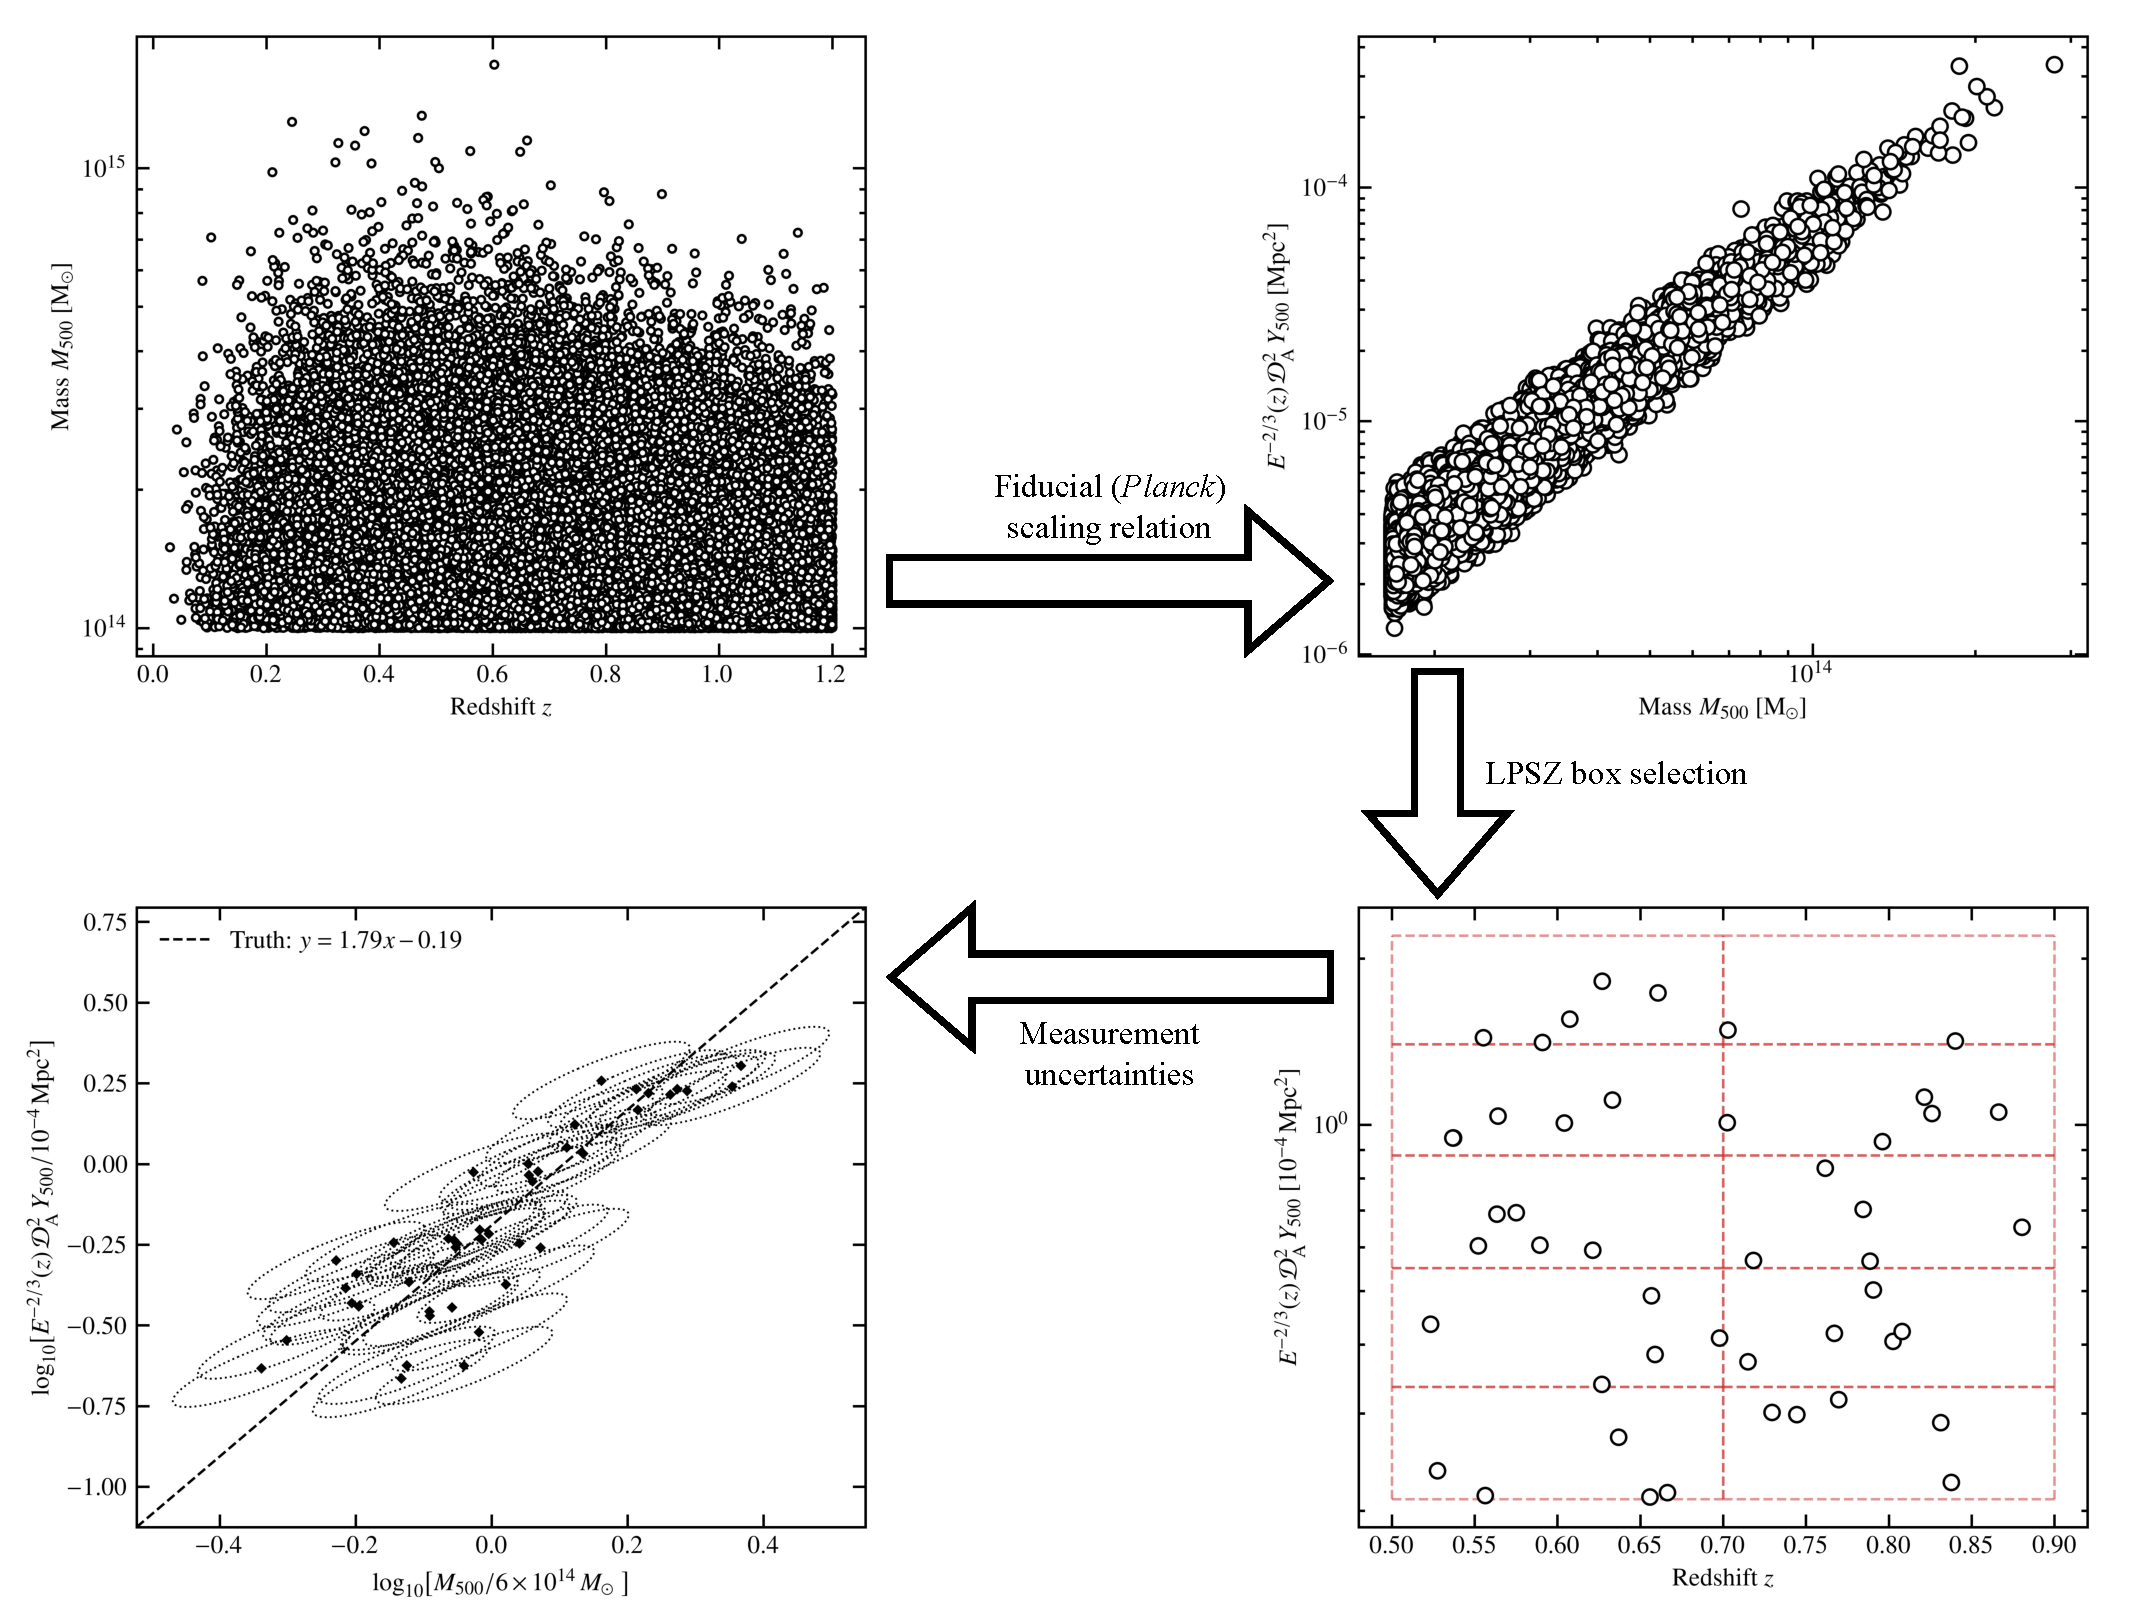
\includegraphics[width=\linewidth]{Figures/Chap_scaling/LPSZ/lpsz_sample_gen.pdf}
    \caption{
        Procédure de génération d'un échantillon d'amas similaire à celui du LPSZ.
        Un échantillon de halos est généré aléatoirement dans le plan $(M_{500}, z)$ à partir d'une fonction de masse donnée (\textit{haut gauche}).
        Une relation d'échelle fiducielle est utilisée pour obtenir des valeurs d'observable SZ correspondantes (\textit{haut droit}).
        Une sélection similaire à celle du LPSZ sur les valeurs d'observable SZ est réalisée pour obtenir un échantillon de 50 amas (\textit{bas droit}).
        Des incertitudes de mesure corrélées sur la masse et sur l'observable sont ensuite générées (\textit{bas gauche}).
        L'ellipse autour de chaque point représente l'intervalle $1\sigma$ de la gaussienne à deux dimensions utilisée comme incertitude.
    }
    \label{fig:scaling:lpsz_sample_gen}
\end{figure*}

Notons que cette procédure ignore un élément important de la fonction de sélection du grand programme SZ, qui est la sélection dans les catalogues \textit{Planck} et ACT.
En ne tenant pas compte des fonctions de sélection de ces deux relevés, nous émettons l'hypothèse que les catalogues d'amas qu'ils ont permis de construire sont représentatifs de la population d'amas dans l'Univers.
Nous ignorons ainsi les mauvaises estimations de masse des amas dues à la présence de bruit corrélé dans les cartes.
Une étude complète se devra de tenir compte de ces effets, afin de ne pas sous-estimer les incertitudes sur les paramètres de la relation d'échelle.

% ------------------------------------------------------------------------------------- %
\subsection{Modélisation et impact de la sélection}
\label{sec:scaling:intercept_bias}

La fonction de sélection du grand programme SZ, reproduite pour générer des échantillons aléatoires, peut avoir un impact sur l'ajustement de la relation d'échelle.
Toutefois, il est difficile de l'inclure dans le modèle bayésien hiérarchique mis en place par \texttt{LIRA}.
Une première idée pourrait être, pour chaque amas, de définir une valeur de seuil en observable correspondant à la limite inférieure de la boîte dans laquelle il a été sélectionné.
La troncature utilisée pour corriger du biais de Malmquist, décrite en section \ref{sec:scaling:malmquist}, pourrait alors être utilisée indépendamment pour chaque boîte.
Cette procédure n'est toutefois pas correcte: il est faux de dire qu'un amas détecté dans une boîte $i$ n'aurait pas pu faire partie de l'échantillon si sa valeur d'observable était inférieure à la limite basse de la boîte, alors qu'il aurait de fait pu être sélectionné dans la boîte inférieure $i-1$.

Une façon de tenir compte de la sélection est donc de considérer une troncature des données à la valeur d'observable définie par la limite inférieure $Y_{\rm low}$ de la boîte de plus basse masse de l'échantillon.
Afin d'évaluer la validité de cette modélisation, la procédure détaillée en \ref{sec:scaling:lpsz_sample_selection} est utilisée pour générer 5000 échantillons fictifs.
La relation d'échelle est ajustée deux fois pour chaque échantillon.
Dans un premier temps, nous ne considérons pas de coupure en observable, ce qui revient à ignorer la sélection en boîtes.
L'ajustement est ensuite réalisé en tenant compte d'une coupure inférieure en observable à la valeur de $Y_{\rm low}$.

\begin{figure*}[t]
    \centering
    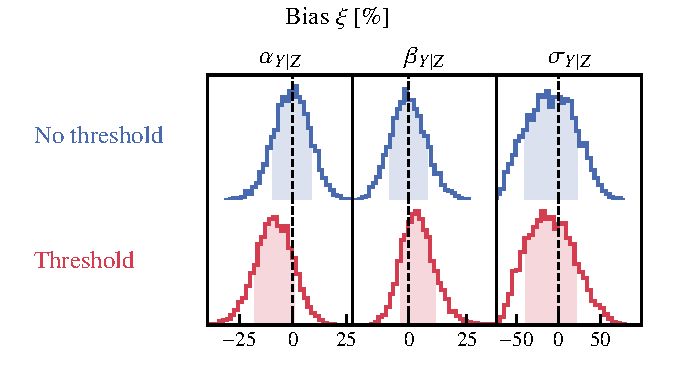
\includegraphics[height=5.3cm]{Figures/Chap_scaling/LPSZ/1_threshold_lowscatt_xi.pdf}
    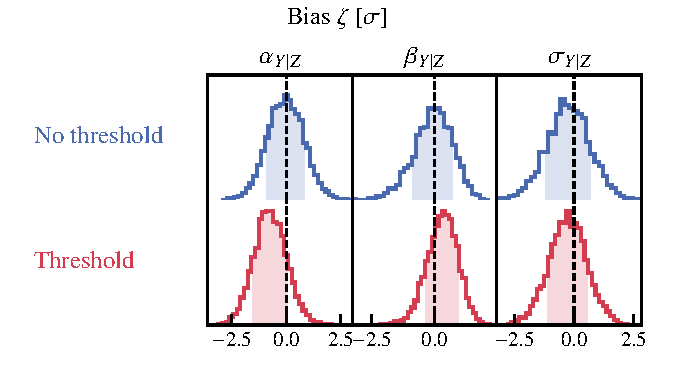
\includegraphics[height=5.3cm, trim={3cm 0 0 0}, clip]{Figures/Chap_scaling/LPSZ/1_threshold_lowscatt_zeta.pdf}
    \caption{
        Distribution des biais $\xi$ (\textit{gauche}) et $\zeta$ (\textit{droite}) sur les trois paramètres d'intérêt de la relation d'échelle pour les 5000 réalisations d'échantillons.
        Les ajustements sont réalisés sans tenir compte de coupure en observable (bleu) et en tenant compte d'une coupure à $Y_{\rm low}$ (rouge).
        Les régions colorées correspondent aux intervalles de confiance à $1\sigma$.
    }
    \label{fig:scaling:zeta_xi_threshold}
    \vspace{10pt}
    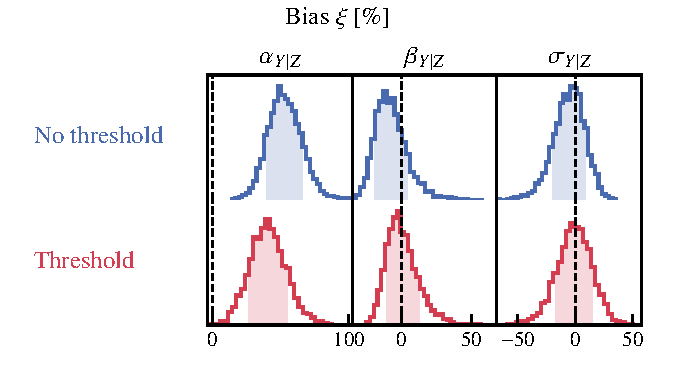
\includegraphics[height=5.3cm]{Figures/Chap_scaling/LPSZ/2_threshold_highscatt_xi.pdf}
    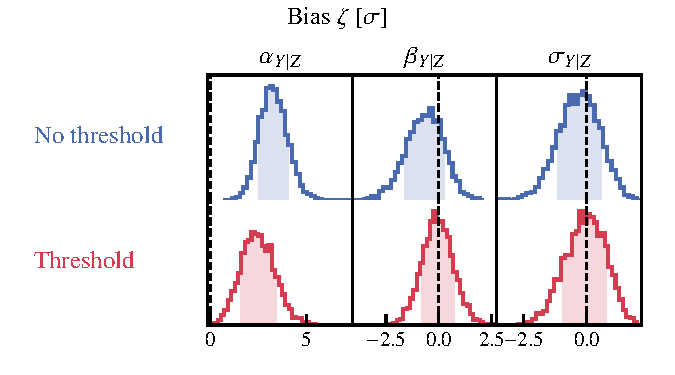
\includegraphics[height=5.3cm, trim={3cm 0 0 0}, clip]{Figures/Chap_scaling/LPSZ/2_threshold_highscatt_zeta.pdf}
    \caption{
        Biais $\xi$ et $\zeta$ sur les paramètres d'intérêt de la relation d'échelle pour une dispersion intrinsèque deux fois supérieure à celle supposée par \textit{Planck} ($\sigma_\yz = 0.15$).
        La légende est identique à celle de la figure \ref{fig:scaling:zeta_xi_threshold}.
    }
    \label{fig:scaling:zeta_xi_threshold_2}
\end{figure*}

Les distributions des valeurs de biais $\xi$ et $\zeta$ pour ces ajustements sont présentées en figure \ref{fig:scaling:zeta_xi_threshold}.
On observe que les résultats ne sont pas biaisés, avec des valeurs moyennes de $\zeta$ de l'ordre de $0.05\sigma$.
Lors de la prise en compte d'une coupure en observable à une valeur de $Y_{\rm low}$, les résultats sont légèrement biaisés ($\zeta \sim 0.5\sigma$).
Ce résultat indique que la fonction de sélection du grand programme SZ n'est pas bien décrite par une coupure en observable à la valeur la plus basse pouvant être sélectionnée pour la construction de l'échantillon.

L'absence de biais pour l'analyse ignorant les effets de sélection est surprenante, car elle semble indiquer que la fonction de sélection complexe du grand programme SZ n'induit aucun biais sur la mesure de la relation d'échelle masse-observable.
Afin de comprendre ce résultat, nous avons répété l'analyse précédente en considérant une valeur de dispersion intrinsèque deux fois plus grande ($\sigma_\yz = 0.15$).
Comme nous l'avons vu en \mypageref{sec:scaling:malmquist}, le biais de Malmquist est conditionné par l'existence d'une dispersion intrinsèque.
En effet, c'est cette dispersion qui permet à certains amas d'être détectés avec une valeur d'observable plus élevée que celle prédite par la relation linéaire masse-observable, ce qui induit une surreprésentation des points au dessus de la relation.
Ainsi, en augmentant la dispersion intrinsèque de la relation, les effets de sélection sont amplifiés, et pourront être plus facilement détectables.

Les résultats de cette analyse sont présentés en figure \ref{fig:scaling:zeta_xi_threshold_2}.
Les effets induits par la sélection de l'échantillon du grand programme SZ y apparaissent très clairement pour cette valeur de dispersion.
Ceux-ci se manifestent sous la forme d'un biais significatif sur l'ordonnée à l'origine de la relation $\alpha_\yz$, avec une valeur moyenne de $\zeta \simeq 3\sigma$.
En revanche, à l'inverse du biais de Malmquist habituel (voir figure \ref{fig:malmquist}), aucun biais significatif n'est détecté sur la pente de la relation $\beta_\yz$.
Le biais sur l'ajustement de la relation d'échelle induit par la fonction de sélection du grand programme SZ est donc singulier.
De plus, la prise en compte des effets de sélection par une coupure en observable ne permet pas de corriger ce biais.

Afin de comprendre l'origine du biais sur l'ordonnée à l'origine de la relation d'échelle, nous pouvons appliquer la même réflexion que celle permettant d'expliquer le biais de Malmquist.
Comme nous l'avons vu en section \mypageref{sec:scaling:malmquist}, le biais de Malmquist est dû à une surreprésentation des points au dessus d'un seuil en observable, qui entraîne une inclinaison de la pente de la relation.
Dans le cas du grand programme SZ, les données sont composées de points sélectionnés en boîtes, créant des surreprésentations régulièrement espacées le long de la relation d'échelle.
Par conséquent, une droite ajustée passant par les régions surreprésentées sera décalée vers le haut, correspondant bien à un biais sur l'ordonnée à l'origine.
Cette interprétation de l'origine du biais est illustrée en figure \ref{fig:scaling:intercept_bias}, comparant les surreprésentations des points dans le cas d'une coupure en observable (gauche) et d'une sélection en boîtes (droite).

\begin{figure*}[t]
    \centering
    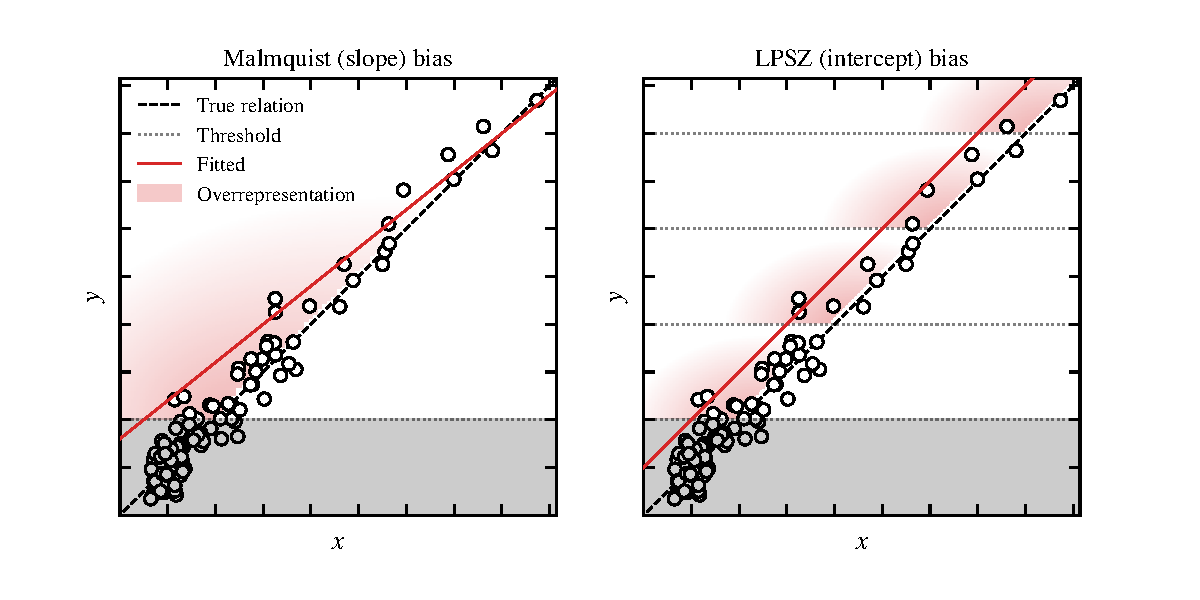
\includegraphics[width=\linewidth]{Figures/Chap_scaling/bias_intercept_illu.pdf}
    \caption{
        Illustration de la cause du biais sur l'ordonnée à l'origine.
        Pour une coupure en observable (\textit{gauche}), une surreprésentation de points au dessus du seuil (région rouge) entraîne une rotation de la relation d'échelle ajustée (droite rouge), et donc un biais sur la pente.
        Pour une sélection en boîtes comme celle du LPSZ (\textit{droite}), des coupures correspondant aux seuils des boîtes créent des surreprésentations au dessus de ces seuils.
        Le résultat est un décalage de la relation d'échelle ajustée, correspondant à un biais sur l'ordonnée à l'origine.
    }
    \label{fig:scaling:intercept_bias}
\end{figure*}

La sélection du LPSZ entraîne donc un biais sur l'ordonnée à l'origine de la relation d'échelle.
La valeur de ce biais dépend de la dispersion intrinsèque autour de la relation d'échelle.
Si la valeur de $\sigma_\yz$ supposée par la collaboration \textit{Planck} \cite{planck_collaboration_planck_2011} est réaliste, le biais est complètement négligeable.
Si cette valeur est sous-estimée, le bais peut être significatif.
Afin de pouvoir arriver à des résultats non-biaisés, il sera possible d'étudier l'évolution de la valeur de ce biais avec la dispersion intrinsèque grâce à des simulations, grâce à la répétition des études présentées dans cette section pour plusieurs valeurs de dispersion intrinsèque.
Comme le montrent les figures \ref{fig:scaling:zeta_xi_threshold} et \ref{fig:scaling:zeta_xi_threshold_2}, les estimations de la dispersion intrinsèque de la relation d'échelle ne sont pas biaisées pour les deux valeurs testées.
Par conséquent, il sera possible de connaître la valeur de la dispersion intrinsèque à l'issue du grand programme SZ, et de corriger la valeur de l'ordonnée à l'origine \textit{ad hoc} grâce aux résultats obtenus sur des simulations.

% ------------------------------------------------------------------------------------- %
\subsection{Incertitudes sur les paramètres d'intérêt}

En plus du biais des estimateurs des paramètres de la relation d'échelle, nous pouvons étudier la dispersion de ces derniers, donnée par la grandeur $\eta$ définie dans l'équation (\ref{eq:scaling:eta}).
Les valeurs obtenues sont une incertitude relative moyenne de 10\% pour les paramètres $\alpha_\yz$ et $\beta_\yz$, et de 34\% pour la dispersion intrinsèque $\sigma_\yz$.
Ces valeurs sont reportées en table \ref{tab:scaling:eta_lpsz}.
De telles incertitudes sont comparables avec celles obtenues pour la même relation d'échelle par la collaboration \textit{Planck} \cite{planck_collaboration_planck_2011}.
Cependant, comme nous l'avons discuté en section \mypageref{sec:scaling:sota}, les incertitudes obtenues dans cette étude ne sont pas directement comparables à celles obtenues ici, car l'analyse bayésienne hiérarchique utilisée propage des incertitudes systématiques qui ne sont pas prises en compte dans l'analyse de \cite{planck_collaboration_planck_2011}.
Il est plus juste de comparer ces résultats avec ceux de CoMaLit \cite{sereno_comparing_2015}, utilisant le même échantillon d'amas que la collaboration \textit{Planck} et une régression similaire à celle utilisée ici.
Les incertitudes de 10\% sur les paramètres d'intérêt représentent une grande amélioration, due à la qualité des contraintes sur $Y_{500}$ et $M_{500}$ attendues dans le cadre du grand programme SZ de NIKA2 et à la couverture en masse de son échantillon.

\begin{table}[t]
    \setlength{\tabcolsep}{20pt}
    \small
    \centering
    \begin{tabular}{c c c}
        \toprule
        Paramètre $\vartheta$ & Distribution \prior &  $\eta_\vartheta$ [\%] \\
        % ========================================================================== %
        \midrule
        \multicolumn{3}{c}{\textit{Analyse de base}} \\
        \midrule
        % -------------------------------------------------------------------------- %
        $\alpha_\yz$ & $\mathcal{U}(-10^4, 10^4)$ & $10.2$ \\
        $\beta_\yz$  & Student $t_1$              & $10.1$ \\
        $\sigma_\yz$ & $\mathcal{U}(0, 10^4)$     & $34.0$ \\
        % ========================================================================== %
        \midrule
        \multicolumn{3}{c}{\textit{Analyse de base + biais hydrostatique}} \\
        \midrule
        % -------------------------------------------------------------------------- %
        $\alpha_\yz$ & $\mathcal{U}(-10^4, 10^4)$ & $232.0$ \\
        $\beta_\yz$  & Student $t_1$              & $11.8$ \\
        $\sigma_\yz$ & $\mathcal{U}(0, 10^4)$     & $35.2$ \\
        $\alpha_{X|Z}$ & $\mathcal{U}(-0.4, 0.4)$ & -- \\
        % ========================================================================== %
        \midrule
        \multicolumn{3}{c}{\textit{Analyse de base + estimateur de masse dispersé}} \\
        \midrule
        % -------------------------------------------------------------------------- %
        $\alpha_\yz$ & $\mathcal{U}(-10^4, 10^4)$ & $14.7$ \\
        $\beta_\yz$  & Student $t_1$              & $16.8$ \\
        $\sigma_\yz$ & $\mathcal{U}(0, 10^4)$     & $45.7$ \\
        $\sigma_{X|Z}$ & $\mathcal{U}(0, 10^4)$   & -- \\
        % ========================================================================== %
        \bottomrule
    \end{tabular}
    \caption{%
        Liste des distributions \prior\ et des incertitudes relatives moyennes $\eta$ pour les paramètres d'intérêt de la relation d'échelle dans le cas du LPSZ.
        Les dispersions des estimateurs des paramètres $\alpha_{X|Z}$ et $\sigma_{X|Z}$ ne sont pas répertoriés car ceux-ci sont des paramètres de nuisance, dont les contraintes ne sont pas l'objectif de l'analyse.
    }
    \label{tab:scaling:eta_lpsz}
\end{table}

L'analyse présentée précédemment fixe certains des paramètres de nuisance inclus dans le modèle hiérarchique utilisé pour la régression.
Comme nous l'avons vu en section \mypageref{sec:scaling:valid}, la présence de ces paramètres dans le modèle augmente la dispersion des estimateurs des paramètres d'intérêt de la relation d'échelle.
Nous cherchons donc à quantifier cette augmentation.

Nous considérons dans un premier temps un biais dans l'estimateur de masse $\alpha_{X|Z}$ (équation \ref{eq:scaling:mass_estim}).
Il s'agit là d'une considération réaliste, puisque les masses utilisées dans le cadre du grand programme SZ sont des masses hydrostatiques, et que celles-ci sont en moyenne affectés d'un biais (voir section \ref{sec:hse_bias}).
L'objectif de cette analyse est d'évaluer la perte en précision des estimateurs des paramètres d'intérêt de la relation d'échelle due à la propagation de l'incertitude sur le biais hydrostatique.
Nous répétons donc notre analyse en considérant une distribution \prior\ non-informative sur $\alpha_{X|Z}$ correspondant à des valeurs sensées du biais hydrostatique $b$, soit une distribution uniforme entre $-0.4$ et $0.4$.
Les résultats sont également présentés en table \ref{tab:scaling:eta_lpsz}.
Les incertitudes sur la pente et la dispersion intrinsèque de la relation d'échelle sont presque inchangées.
Cependant, l'incertitude sur l'ordonnée à l'origine est augmentée d'un facteur supérieur à 20.
Les données du grand programme SZ n'apportent pas de contraintes sur le biais hydrostatique; par conséquent, c'est la distribution \prior\ sur ce paramètre qui domine.
Il sera donc nécessaire d'adopter un \prior\ informatif pour l'ajustement de la relation d'échelle du grand programme SZ, sans quoi l'un des paramètres d'intérêt ne sera pas contraint.

Enfin, nous répétons l'analyse en considérant un estimateur de masse non-biaisé, mais dispersé, soit $\sigma_{X|Z} \neq 0$.
L'objectif est ici d'évaluer la perte de précision due à la propagation de l'incertitude sur la dispersion de l'estimateur de masse hydrostatique.
Les résultats sont présentés en table \ref{tab:scaling:eta_lpsz}.
Les incertitudes sur les paramètres d'intérêt sont augmentées, de $\sim$ 10\% à $\sim$ 15\% pour l'ordonnée à l'origine et la pente, et de 34\% à 46\% pour la dispersion intrinsèque.
L'augmentation est significative, mais les incertitudes obtenues restent toutefois plus faibles que celles obtenues par les travaux précédents sur les données \textit{Planck}.
Là encore, un \prior\ informatif sur la dispersion de l'estimateur de masse permettrait de réduire le volume de l'espace des paramètres, et donc les incertitudes sur les paramètres d'intérêt.
Une telle connaissance peut être obtenue par l'étude d'amas simulés, en comparant la masse réelle des amas et celle obtenue par combinaison de leurs profils de pression et de densité (voir par exemple \cite{gianfagna_exploring_2021}).

% ------------------------------------------------------------------------------------- %
\subsection{Extensions du grand programme SZ}

Comme nous l'avons vu en section \mypageref{sec:lpsz}, le grand programme SZ de NIKA2 dispose de 300 heures d'observations avec NIKA2, attribuées à la collaboration pour la construction de l'instrument.
La caméra NIKA2 étant aujourd'hui à disposition de la communauté scientifique, il est possible de soumettre des propositions pour obsrver d'autres amas que ceux présents au sein de l'échantillon du LPSZ.
La possibilité d'observer un échantillon d'amas complémentaire au LPSZ est donc envisagée.
Dans cette section, nous nous intéressons à l'apport de telles extensions au programme, du point de vue des contraintes sur la relation d'échelle masse-observable.
Pour cela, nous répétons l'analyse présentée précédemment pour des échantillons combinant le LPSZ et d'autres amas, en considérant différentes sélections.

\subsubsection{Augmentation de la taille d'échantillon} % ----------------------------- %

La première extension considérée est une augmentation du nombre d'amas par boîte dans l'échantillon du LPSZ, en considérant la même sélection que pour l'échantillon réel.
Nous avons vu que le LPSZ comportait cinq amas par boîte; nous répétons donc l'analyse pour un échantillon de taille multipliée par deux, trois, puis quatre.
L'incertitude relative $\eta$ sur les paramètres d'intérêt, définie par l'équation (\ref{eq:scaling:eta}), est calculée et comparée à celle pour l'analyse de base, afin d'évaluer le gain associé à ces augmentations d'échantillon.

Les résultats sont présentés en bleu sur la figure \ref{fig:scaling:eta_ext}.
On observe une diminution de l'incertitude sur les paramètres avec l'augmentation du nombre d'amas, qui correspond à une diminution de l'erreur statistique.
En revanche, on remarque que cette diminution est faible, avec une erreur relative passant de 10\% pour le LPSZ nominal (cinq amas par boîtes) à $\sim$7.5\% pour une multiplication par quatre de la taille de l'échantillon.
Ce gain est très faible en regard du temps d'observation nécessaire à son obtention, puisqu'il exigerait une proposition de temps ouvert de 900 heures d'observation.
Nous en déduisons qu'une extension réaliste du programme en considérant la même sélection ne serait pas bénéfique du point de vue de la précision de l'estimation de la relation d'échelle.

\begin{figure*}[t]
    \centering
    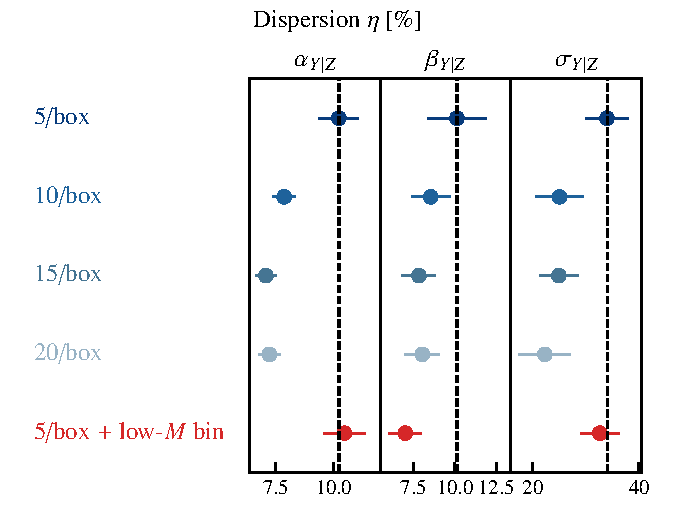
\includegraphics[width=.6\linewidth]{Figures/Chap_scaling/eta_ext.pdf}
    \caption{
        Évolution de l'incertitude relative sur les paramètres d'intérêt avec les extensions du grand programme SZ: ajout d'amas avec la même fonction de sélection (bleu) et ajout d'amas de 10 amas de basse masse (rouge).
    }
    \label{fig:scaling:eta_ext}
\end{figure*}

\subsubsection{Extension à basse masse} % --------------------------------------------- %

S'il n'est pas réaliste d'améliorer les contraintes mises par le LPSZ sur la relation d'échelle en augmentant simplement le nombre d'amas présents dans ce dernier, il reste possible de considérer une sélection différente.
Par exemple, il est possible d'observer des amas en dehors de la gamme de masse et de redshift de l'échantillon de base.
Une extension en redshift n'apporterait que peu de contraintes supplémentaires mesurables dans cette étude.
En effet, nous n'avons pas considéré la mesure de l'évolution avec le redshift de la relation d'échelle.
Ainsi, ajouter des amas à bas (ou haut) redshift sur la même gamme de masse que celle couverte par l'échantillon du LPSZ reviendrait simplement à un ajout d'amas dans l'échantillon, et nous avons vu précédemment que le gain en précision serait minime.

En revanche, il est possible d'étendre la gamme de masse couverte.
Étant donné le peu d'amas de masse supérieure à $10^{15} \; M_\odot$ dans l'Univers (voir figure \ref{fig:cluster_catalogs_mz}), une extension à haute masse semble irréaliste.
Nous considérons donc une extension à basse masse de l'échantillon du LPSZ, en ajoutant un intervalle en observable SZ.
Cette extension est illustrée en figure \ref{fig:scaling:lpsz_lowm}.
Elle correspond à l'ajout de deux boîtes à faibles valeurs de $Y$, une pour chaque intervalle en redshift de l'échantillon, comportant cinq amas chacune.
L'extension représente alors seulement dix amas, soit bien moins que les 150 nécessaires à multiplier la taille de l'échantillon par quatre.

Les incertitudes relatives sur les paramètres de la relation d'échelle pour 5000 réalisations d'échantillons comportant cette extension sont présentées en rouge sur la figure \ref{fig:scaling:eta_ext}.
On voit que les incertitudes sur l'ordonnée à l'origine et la dispersion intrinsèque de la relation sont inchangées par rapport à l'analyse de base (ligne noire pointillée).
En revanche, l'incertitude sur la pente $\beta$ est diminuée, atteignant une valeur moyenne de $\sim$7\%.
Ce gain correspond à une couverture étendue en masse, permettant de mieux ajuster la pente de la relation.
Le suivi de dix amas de basse masse pourrait donc améliorer les contraintes mises par le LPSZ sur la relation d'échelle, en plus d'études intéressantes sur les propriétés physiques de ces objets \cite{keruzore_exploiting_2020}.
Il est toutefois à noter que si de tels amas existent (par exemple dans le dernier catalogue ACT \cite{hilton_atacama_2021}, voir figure \ref{fig:cluster_catalogs_mz}), le temps nécessaire pour observer des amas de basse masse est important.
Il sera donc nécessaire de calculer le temps d'observation requis, pour éventuellement construire un échantillon de moins de dix amas.

\begin{figure*}[t]
    \centering
    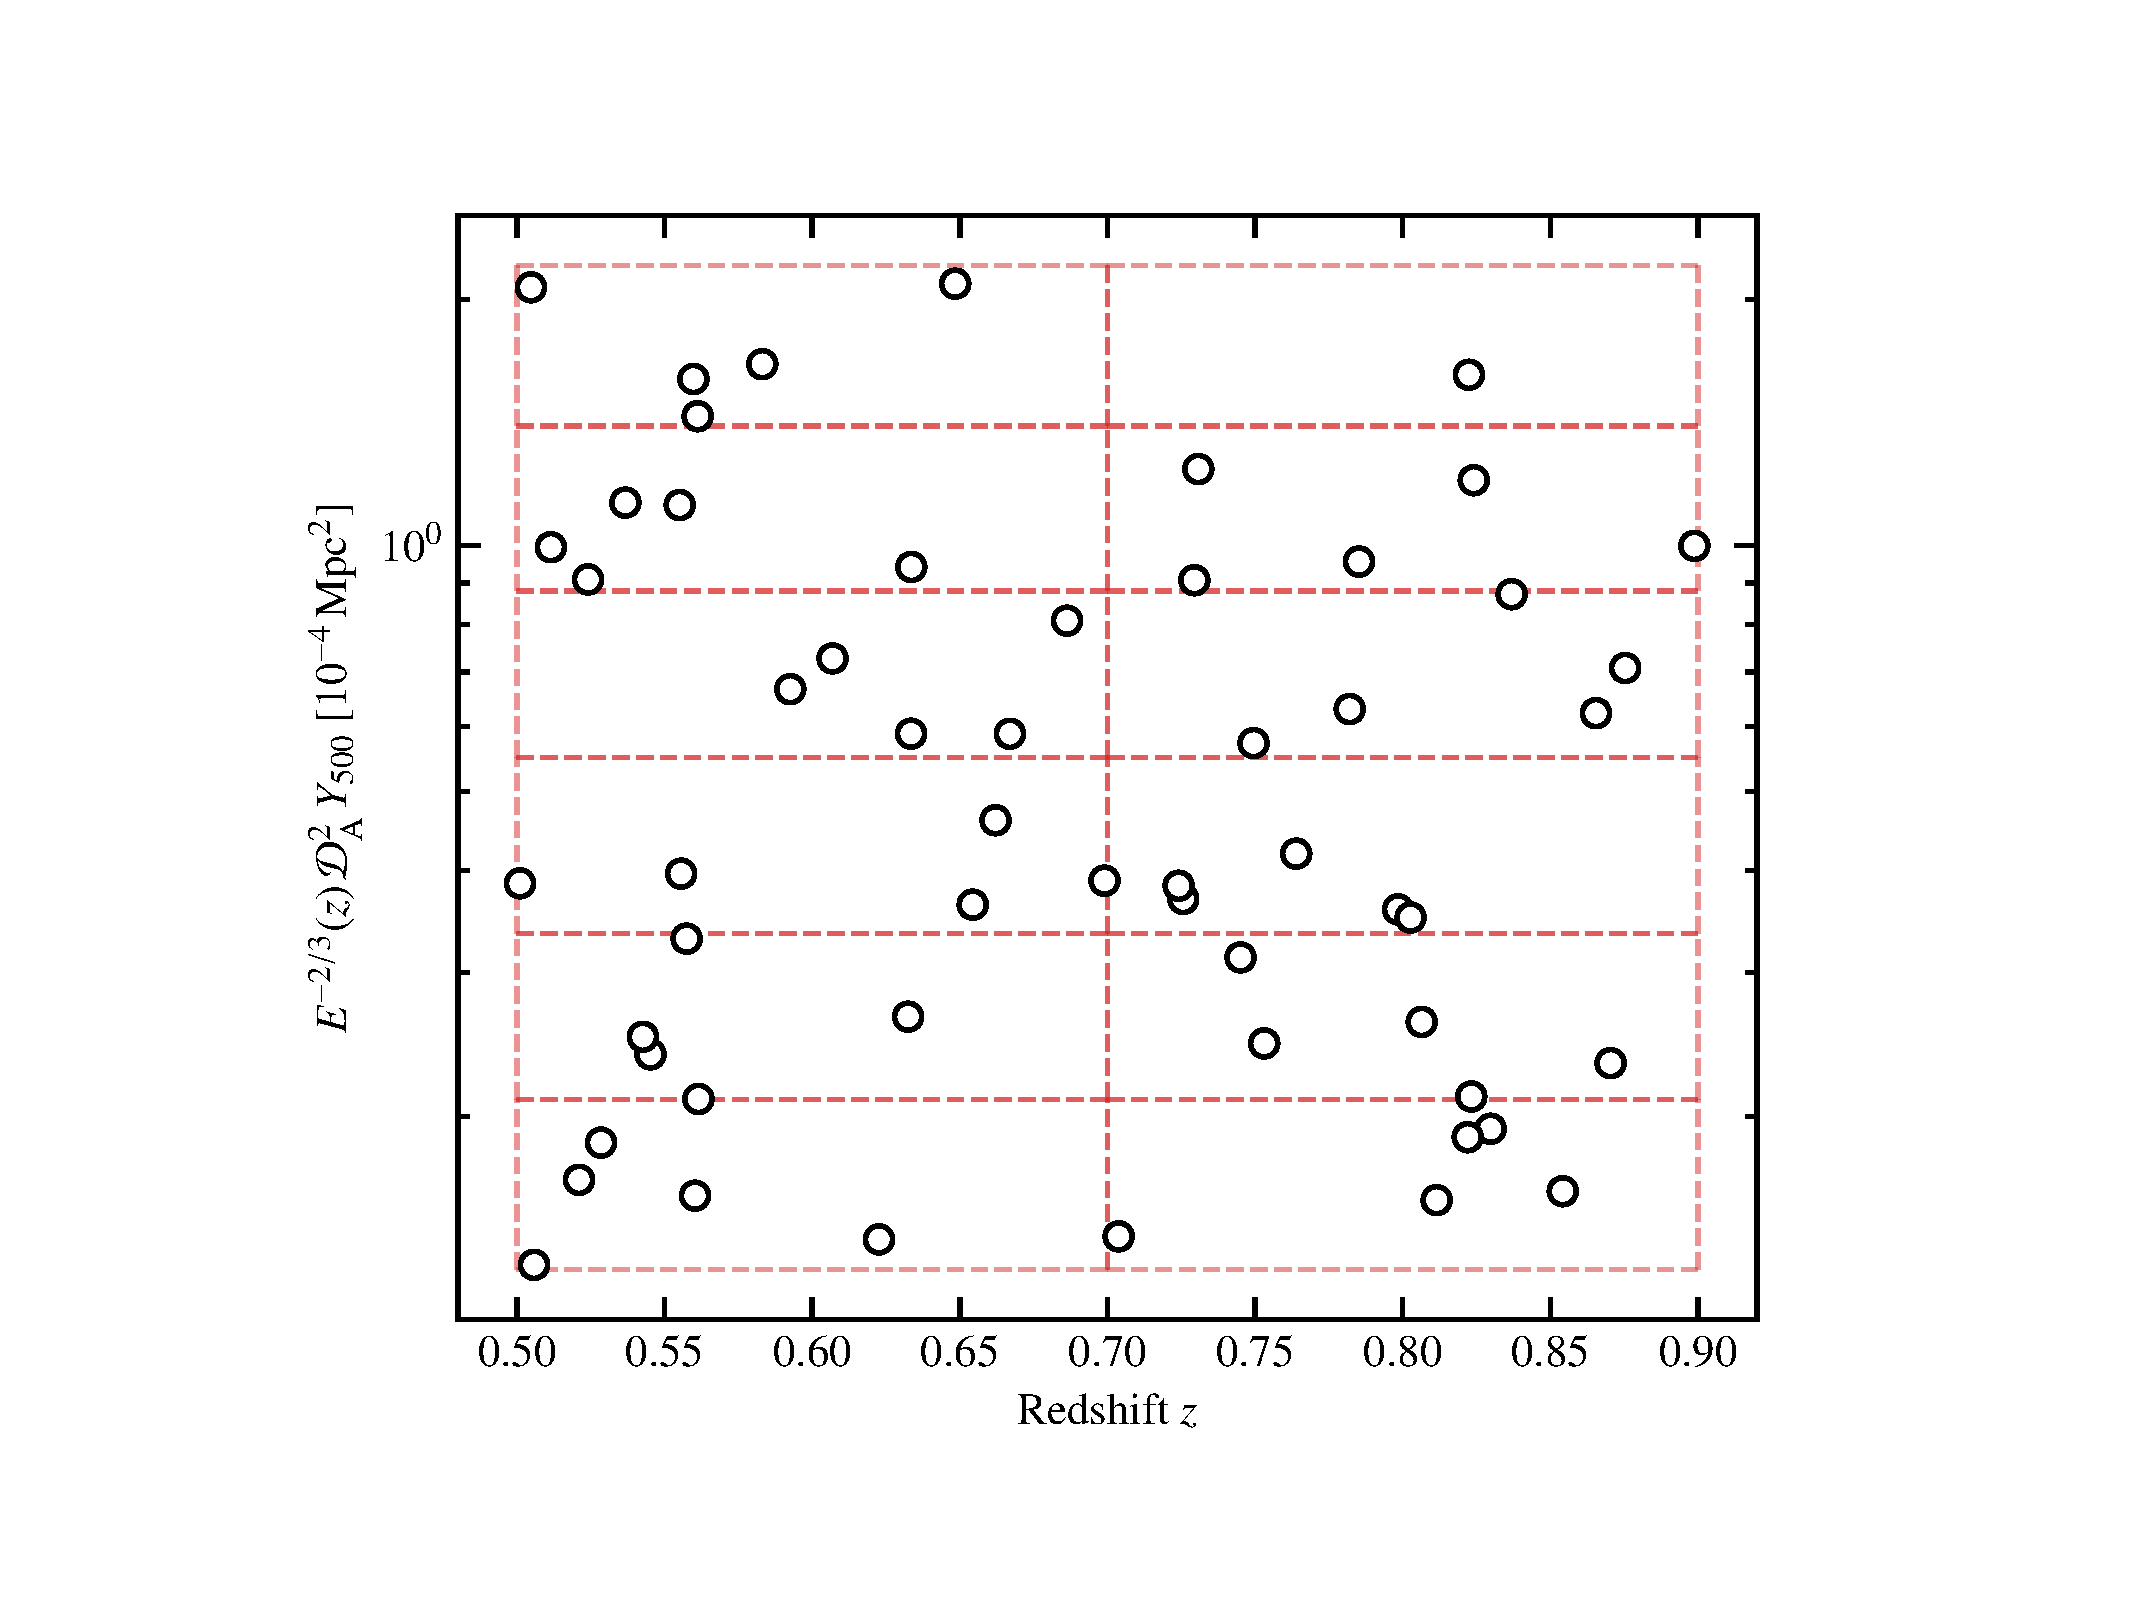
\includegraphics[width=.6\linewidth]{Figures/Chap_scaling/lowm_bin.pdf}
    \caption{
        Exemple d'échantillon combinant celui du grand programme SZ (voir figure \ref{fig:lpsz_sample}) et une extension à basse masse.
        Deux boîtes (bas redshift et haut redshift) sont ajoutées correspondant à des faibles valeurs d'observable $Y$.
    }
    \label{fig:scaling:lpsz_lowm}
\end{figure*}

% ===================================================================================== %
\section{Conclusions et perspectives}

Dans ce chapitre, nous avons présenté la relation d'échelle liant le paramètre de Compton intégré $Y_{500}$ et la masse $M_{500}$, son origine physique, et sa modélisation statistique.
Nous avons mis en place une analyse basée sur un modèle bayésien hiérarchique, consistant en une combinaison structurelle de plusieurs sous-modèles répondant chacun à un effet systématique pouvant affecter l'ajustement de cette relation.
La validation de l'algorithme a montré que ce modèle pouvait prendre en compte ces systématiques afin de livrer des estimations non-biaisées des paramètres d'intérêt de la relation d'échelle.
Enfin, l'application à des jeux de données simulés réalistes similaires au grand programme SZ de NIKA2 nous a permis d'identifier un biais dû à la fonction de sélection de ce dernier, analogue au biais de Malmquist.
Nous avons vu que ce biais pouvait être significatif dans le cas d'une dispersion intrinsèque importante autour de la relation d'échelle.
Enfin, nous avons pu évaluer les incertitudes sur les paramètres d'intérêt de la relation.
Si les observations du grand programme SZ permettent d'atteindre la qualité de données attendue, celui-ci permettra un gain en précision sur la connaissance de la relation d'échelle par rapport aux analyses des données \textit{Planck}, avec une prise en compte plus complète des systématiques affectant l'analyse.

Afin de renforcer ces conclusions, certains axes d'approfondissement peuvent être envisagés pour cette étude.
Lors de la génération d'échantillons simulés, nous n'avons pas tenu compte des diverses systématiques associées aux catalogues d'amas d'entrée.
En effet, l'échantillon du grand programme SZ a été construit à partir des catalogues \textit{Planck} et ACT d'amas de galaxies, et ceux-ci ne représentent pas une mesure parfaite de l'Univers.
Par exemple, plusieurs contaminations peuvent affecter la mesure du paramètre de Compton intégré d'un amas avec \textit{Planck}: des sources ponctuelles non-résolues, une anisotropie primaire du CMB, ou simplement du bruit instrumental.
Ces sources d'incertitude n'ont pas été prises en compte au cours de cette étude, et pourraient impacter les contraintes sur la relation d'échelle avec le LPSZ.

D'autre part, comme nous l'avons vu au cours de ce chapitre, un biais de sélection peut affecter l'estimation de la relation d'échelle avec le grand programme SZ.
Une piste pour corriger ce biais serait d'étudier sa dépendance avec les paramètres de la relation.
Répéter l'étude présentée dans ce chapitre pour différentes valeurs de dispersion intrinsèque permettrait de quantifier l'évolution du biais avec ce paramètre, et donc de pouvoir mettre en place une correction \textit{ad-hoc} pour les résultats finaux du grand programme SZ, en fonction de la valeur de dispersion mesurée lors de l'ajustement des données réelles.

Nous avons vu que la procédure d'ajustement du modèle bayésien hiérarchique permettait de tenir compte d'un grand nombre d'effets systématiques en introduisant des paramètres de nuisance.
Cependant, si cette procédure permet d'obtenir une propagation complète des incertitudes sur les résultats finaux, elle implique par construction une augmentation de ces incertitudes.
La question des \prior\ sur les paramètres de nuisance est donc centrale.
Afin de pouvoir concilier une propagation complète de toutes les incertitudes systématiques et une mesure précise de la relation d'échelle, il sera nécessaire d'imposer des \prior\ informatifs sur les paramètres de nuisance comme le biais et la dispersion de l'estimateur de masse hydrostatique.
Ces \prior\ pourront être mesurés en combinant le LPSZ avec des données externes (par exemple en optique avec des mesures de masse dynamique ou par dispersion de vitesses), ou en utilisant des simulations hydrodynamiques.

Enfin, l'étude développée a été utilisée pour commencer à prévoir une extension du grand programme SZ pouvant améliorer le pouvoir de contrainte de ce dernier sur la relation d'échelle.
Nous avons vu que multiplier la taille de l'échantillon par deux, trois ou quatre demandait des temps d'observations beaucoup trop importants pour les améliorations atteignables.
En revanche, nous avons aussi montré que le suivi avec NIKA2 d'un échantillon d'amas de faible masse permettrait une amélioration conséquente des contraintes sur la pente de la relation avec seulement dix amas.
Ce résultat pourra être utilisé pour justifier une demande de temps d'observation avec NIKA2.
